%% The following is a directive for TeXShop to indicate the main file
%%!TEX root = ../../thesis.tex

\chapter{Modelling electromagnetics on cylindrical meshes}
\label{ch:casing-software}

A number of geophysical electromagnetic (EM) problems lend themselves to cylindrical geometries. Airborne EM problems over a 1D layered earth or borehole-logging applications fall into this category; in these cases cylindrical modelling, which removes a degree of freedom in the azimuthal component, can be advantageous as it reduces the computation load. This is useful when running an inversion where many forward modellings are required, and it  is also valuable when exploring and building up an understanding of the behaviour of electromagnetic fields and fluxes in a variety of settings, such as the canonical model of an airborne EM sounding over a sphere, as it reduces feedback time between asking a question and visualizing results (e.g. \cite{Oldenburg2017}).

Beyond these simple settings, there are also a range of scenarios where the footprint of the survey is primarily cylindrical, but 2D or 3D variations in the physical property model may be present. For example if we consider a single sounding in an Airborne EM survey, the primary electric fields are rotational and the magnetic fields are poloidal, but the physical property model may have lateral variations or compact targets. More flexibility is required from the discretization to capture these features. In this case, a 3D cylindrical geometry, which incorporates azimuthal discretization may be advantageous. It allows finer discretization near the source where we have the most sensitivity and the fields are changing rapidly. Far from the source, the discretization is coarser, but it still conforms to the primary behaviour of the EM fields and fluxes and captures the rotational electric fields and poloidal magnetic flux.

In other cases, the most significant physical property variations may conform to a cylindrical geometry, for example in settings where vertical metallic well-casings are present, or in the emerging topic of using geophysics to ``look ahead'' of a tunnel boring machine. Of particular interest to the thesis is understanding the behavior of electromagnetic fields and fluxes in the presence of steel-cased wells. In addition to the hydraulic fracturing application, understanding EM in settings with steel-cased wells is of interest across a range of applications, from characterizing lithologic units with well-logs \citep{Kaufman1990, Kaufman1993, Augustin1989}, to identifying marine hydrocarbon targets \citep{Kong2009, Swidinsky2013, Tietze2015}, to mapping changes in a reservoir induced by hydraulic fracturing or carbon capture and storage \citep{Pardo2013, Borner2015, Um2015, Weiss2016, hoversten2017borehole, Zhang2018}. Carbon steel, a material commonly used for borehole casings, is highly electrically conductive ($10^6 - 10^7$ S/m) and has a significant magnetic permeability ($\geq 100$ $\mu_0$) \citep{wuhabashy1994}; it therefore can have a significant influence on electromagnetic signals. The large contrasts in physical properties between the casing and the geologic features of interest, along with the large range of scales that need to be considered to model both the millimeter-thick casing walls while also capturing geologic features, provide interesting challenges and context for electromagnetics in cylindrical geometries.

In this chapter, I introduce an approach and associated open-source software implementation for simulating Maxwell's equations over conductive, permeable models on 2D and 3D cylindrical meshes. The software is written in Python \citep{van1995python} and is included as an extension to the SimPEG ecosystem \citep{Cockett2015}; Appendix \ref{app:simpegem} provides a description of the SimPEG electromagnetic module. Within the context of current research connected to steel-cased wells, my aim with the development and distribution of this software is two-fold: (1) to facilitate the exploration of the physics of EM in these large-contrast settings, and (2) to provide a simulation tool that can be used for testing other EM codes. The large physical property contrasts in both conductivity and permeability means the physics is complicated and often non-intuitive; as such, we prioritize the ability of the researcher to access and visualize fields, fluxes, and charges in the simulation domain. This is particularly useful when the software is used in conjunction with Jupyter notebooks which facilitate exploration of numerical results \citep{Perez2015}. As the mesh conforms to the geometry of a vertical borehole, a fine discretization can be used in its vicinity without resulting in a onerous computation. This provides the opportunity to build an understanding of the physics of EM in settings with vertical boreholes prior to moving to settings with deviated and horizontal wells. I demonstrate the software with examples at DC, in the frequency domain, and in the time domain. Source-code for all examples is provided as Jupyter notebooks as outlined in Appendix \ref{app:code_list}; they are licensed under the permissive MIT license with the hope of reducing the effort necessary by a researcher to compare to or build upon this work.

This chapter is organized in the following manner. In section \ref{sec:numerical_tools}, I introduce the governing equations, Maxwell's equations, and describe their discretization in cylindrical coordinates. I then compare our numerical implementation to the finite element and finite difference results shown in \citep{Commer2015} as well as a finite volume OcTree simulation described in \citep{Haber2007}. Section \ref{sec:numerical_examples} contains numerical examples of the DC, frequency domain EM, and time domain EM implementations. The two DC resistivity examples (sections \ref{sec:dc_resistivity_part1} and \ref{sec:dc_resistivity_part2}) are built upon the foundational work in \citep{Kaufman1990, Kaufman1993} which use asymptotic analysis to draw conclusions about the behavior of the electric fields, currents, and charges for a well where an electrode has been positioned along its axis.  The final two examples, in sections \ref{sec:FDEM_part1} and \ref{sec:FDEM_part2}, consider a frequency domain experiment inspired by \citep{Augustin1989}. These examples demonstrate the impact of magnetic permeability on the character of the magnetic flux within the vicinity of the borehole and discusses the resulting magnetic field measurements made within a borehole.
\section{Numerical tools}
\label{sec:numerical_tools}

The governing equations under consideration are Maxwell's equations. I provided an overview in Section \ref{sec:background-em}. This section is meant to provide a brief review and set the context for what is required of our numerical tools.

Under the quasi-static approximation, Maxwell's equations are given by:
\begin{equation}
\begin{split}
\nabla \times \vec{e} &= -\frac{\partial \vec{b}}{\partial t} \\
\nabla \times \vec{h} - \vec{j} &= \vec{s}_e
\end{split}
\label{eq:MaxwellTime}
\end{equation}

where $\vec{e}$ is the electric field, $\vec{b}$ is the magnetic flux density, $\vec{h}$ is the magnetic field, $\vec{j}$ is the current density and $\vec{s_e}$ is the source current density. Maxwell's equations can also be formulated in the frequency domain, using the $e^{i \omega t}$ Fourier Transform convention, they are
\begin{equation}
\begin{split}
\nabla \times \vec{E} + i\omega\vec{B} &= 0 \\
\nabla \times \vec{H} - \vec{J} &= \vec{S}_e
\end{split}
\label{eq:MaxwellFreq}
\end{equation}

The fields and fluxes are related through the physical properties: electrical conductivity ($\sigma$, or its inverse, resistivity $\rho$) and magnetic permeability ($\mu$), as described by the constitutive relations
\begin{equation}
\begin{split}
\vec{J} = \sigma \vec{E} \\
\vec{B} = \mu \vec{H}
\end{split}
\label{eq:ConstitutiveRelations}
\end{equation}

At the zero-frequency limit, we also consider the DC resistivity experiment, described by
\begin{equation}
\begin{split}
\nabla \cdot \vec{j} &= I\left(\delta(\vec{r} - \vec{r}_{s^{+}}) - \delta(\vec{r} - \vec{r}_{s^{-}})\right) \\
\vec{e} &= - \nabla \phi
\end{split}
\label{eq:DCequations}
\end{equation}

where $I$ is the magnitude of the source current density, $\vec{r}_{s^+}$ and $\vec{r}_{s^-}$ are the locations of the current electrodes, and $\phi$ is the scalar electric potential.

Of our numerical tools, we require the ability to simulate large electrical conductivity contrasts, include magnetic permeability, and solve Maxwell's equations at DC, in frequency and in time in a computationally tractable manner. Finite volume methods are advantageous for modelling large physical property contrasts as they are conservative and the operators ``mimic'' properties of the continuous operators, that is, the edge curl operator is in the null space of the face divergence operator, and the nodal gradient operator is in the null space of the edge curl operator \citep{Hyman1999}. As such, they are common practice for many electromagnetic simulations (e.g. \cite{Horesh2011, Haber2014, Jahandari2014} and references within), and will be my method of choice.
\subsection{Discretization}
To represent a set of partial differential equations on the mesh, I use a staggered-grid approach \citep{Yee1966} and discretize fields on edges, fluxes on faces, and physical properties at cell centers, as shown in Figure \ref{fig:CylFiniteVolume}. Scalar potentials can be discretized at cell centers or nodes. I consider both cylindrically symmetric meshes and fully 3D cylindrical meshes; the anatomy of a finite volume cell for these scenarios is shown in Figure \ref{fig:CylFiniteVolume} (b) and (c).


\begin{figure}
    \begin{center}
    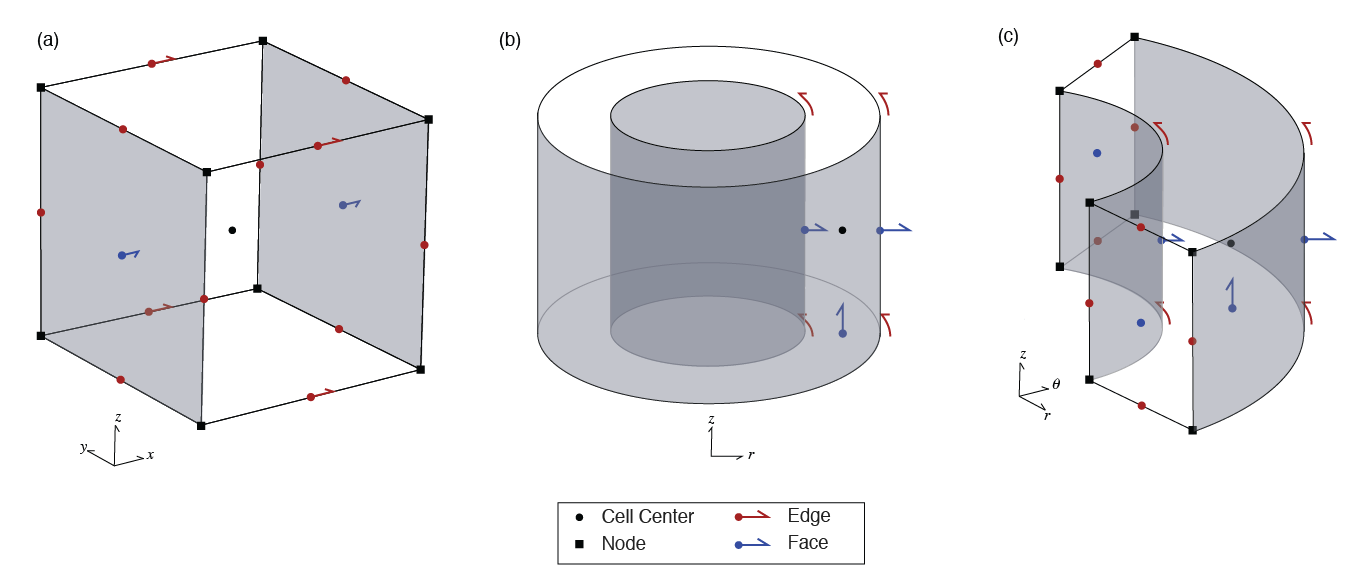
\includegraphics[width=\columnwidth]{figures/casing_software/finiteVolume-02.png}
    \end{center}
\caption{
    Anatomy of a finite volume cell in a (a) cartesian,
    regtangular mesh, (b) cylindrically symmetric mesh, and
    (c) a three dimensional cylindrical mesh.
}
\label{fig:CylFiniteVolume}
\end{figure}


To discretize Maxwell's equations in the time domain (equation \ref{eq:MaxwellTime}) or in the frequency domain (equation \ref{eq:MaxwellFreq}), I invoke the constitutive relations to formulate our system in terms of a single field and a single flux. This gives a system in either the electric field and magnetic flux (E-B formulation), or the magnetic field and the current density (H-J formulation). For example, in the frequency domain, the E-B formulation is
\begin{equation}
    \begin{split}
        \mathbf{C} \mathbf{e} + i\omega\mathbf{b} &= \mathbf{s_m} \\
        \mathbf{C}^\top \mathbf{M}_{\boldsymbol{\mu}^{-1}}^f \mathbf{b} - \mathbf{M}_{\boldsymbol{\sigma}}^e \mathbf{e} &= \mathbf{s_e}
    \end{split}
    \label{eq:DiscreteFDEMEB}
\end{equation}

and the H-J formulation is
\begin{equation}
    \begin{split}
        \mathbf{C}^\top \mathbf{M}_{\boldsymbol{\rho}}^f \mathbf{j} + i\omega\mathbf{M}_{\boldsymbol{\mu}}^e\mathbf{h} &= \mathbf{0} \\
        \mathbf{C} \mathbf{h} - \mathbf{j} &= \mathbf{s_e}
    \end{split}
    \label{eq:DiscreteFDEMHJ}
\end{equation}

where $\mathbf{e}, \mathbf{b}, \mathbf{h}, \mathbf{j}$ are vectors of the discrete EM fields and fluxes; $\mathbf{s_m}$ and $\mathbf{s_e}$ are the discrete magnetic and electric source terms, respectively; $\mathbf{C}$ is the edge curl operator, and the matrices $\mathbf{M}_{\text{prop}}^{e,f}$ are the edge / face inner product matrices. In particular, variable electrical conductivity and variable magnetic permeability are captured in the discretization. The time domain equations are discretized in the same manner; for time-stepping, a first-order backward Euler approach is used. Although the midpoint method, which is second-order accurate, could be considered, it is susceptible to oscillations in the solution, which reduce the order of accuracy, unless a sufficiently small time-step is used \citep{Haber2004, Haber2014}.  Appendix \ref{app:simpegem} provides more details on the discretization of Maxwell's equations in both the frequency and time-domains.

At the zero-frequency limit, each formulation has a complementary discretization for the DC equations. For the E-B formulation the discretization leads to a nodal discretization of the electric potential $\boldsymbol{\phi}$, giving
% \begin{equation}
%     \mathbf{G}^\top \mathbf{M}_{\boldsymbol{\sigma}}^e \mathbf{G} \boldsymbol{\phi} = \mathbf{q}
%     \label{eq:DiscreteDCNodal}
% \end{equation}
\begin{equation}
    \begin{split}
        - \mathbf{G}^\top \mathbf{M}_{\boldsymbol{\sigma}}^e \mathbf{e} &= \mathbf{q} \\
        \mathbf{e} &= -\mathbf{G}\boldsymbol{\phi}
    \end{split}
    \label{eq:DiscreteDCNodal}
\end{equation}

where $\mathbf{G}$ is the nodal gradient operator, and $\mathbf{q}$ is the source term, defined on nodes. Note that the nodal gradient takes the discrete derivative of nodal variables, and thus the output is on edges. The H-J formulation leads naturally to a cell centered discretization of the electric potential
\begin{equation}
    \begin{split}
        \mathbf{V} \mathbf{D}  \mathbf{j} &= \mathbf{q} \\
        \mathbf{M}_{\boldsymbol{\rho}}^f \mathbf{j} &= \mathbf{D}^\top \mathbf{V} \boldsymbol{\phi}
    \end{split}
    \label{eq:DiscreteDCCC}
\end{equation}

Where $\mathbf{D}$ is the face divergence operator, $\mathbf{V}$ is a diagonal matrix of the cell volumes, $\mathbf{q}$ is the source term, which is  defined at cell centers as is $\boldsymbol{\phi}$. Here, the face divergence takes the discrete derivative from faces to cell centers, thus its transpose takes a variable from cell centers to faces. For a tutorial on the finite volume discretization of the DC equations, see \citep{Cockett2016}.

For the EM simulations, natural boundary conditions are employed; in the E-B formulation, this means $\vec{B}\times\vec{n} = 0\vert_{\partial \Omega}$, and in the H-J formulation, we use $\vec{J}\times\vec{n} = 0\vert_{\partial \Omega}$. Within the DC simulations, there is flexibility on the choice of boundary conditions employed. In the simplest scenario, for the nodal discretization, we use Neumann boundary conditions, $\sigma\vec{E} \cdot \vec{n} = 0\vert_{\partial \Omega}$, and for the cell centered discretization, we use Dirichlet boundary conditions $\phi = 0\vert_{\partial \Omega}$.

When employing a cylindrical mesh, the distinction between where the electric and magnetic contributions are discretized in each formulation has important implications. If we consider the cylindrically symmetric mesh (Figure \ref{fig:CylFiniteVolume}b) and a magnetic dipole source positioned along the axis of symmetry (sometimes referred to as the TE mode), we must use the E-B formulation of Maxwell's equation to simulate the resulting toroidal magnetic flux and rotational electric fields. If instead, a vertical current dipole is positioned along the axis of symmetry (also referred to as the TM mode), then the H-J formulation of Maxwell's equations must be used in order to simulate toroidal currents and rotational magnetic fields. The advantage of a fully 3D cylindrical mesh is that it provides additional degrees of freedom, with the discretization in the azimuthal direction. This allows us to simulate more complex responses. However, in order to avoid the need for very fine discretization in the azimuthal direction, we should select the most natural formulation of Maxwell's equations given the source geometry being considered. For a vertical steel cased well and a grounded source, we expect the majority of the currents to flow vertically and radially, thus the more natural discretization to employ is the H-J formulation of Maxwell's equations.

\cite{Haber2014} provides derivations and discussion of the differential operators and inner product matrices; though they are described for a cartesian coordinate system and a rectangular grid, the extension to a three dimensional cylindrical mesh is straightforward. Effectively, a cartesian mesh is wrapped so that the $x$ components become $r$ components, and $y$ components become $\theta$ components, as shown in Figure \ref{fig:cylwrap}.


\begin{figure}
    \begin{center}
    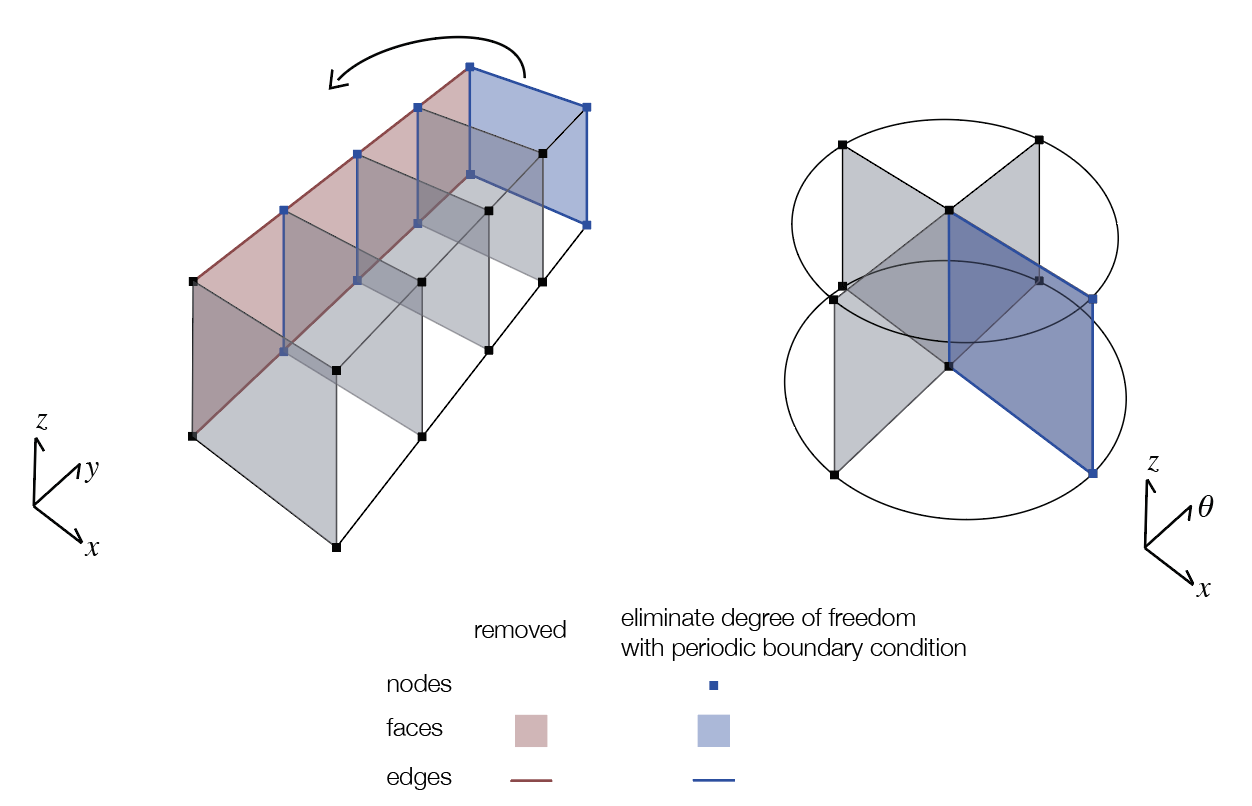
\includegraphics[width=0.9\columnwidth]{figures/cylwrap.png}
    \end{center}
\caption{Construction of a 3D cylindrical mesh from a cartesian mesh.}
\label{fig:cylwrap}
\end{figure}


The additional complications that are introduced are: (1) the periodic boundary condition introduced on boundary faces and edges in the azimuthal direction, (2) the removal of radial faces and azimuthal edges along the axis of symmetry, and (3) the elimination of the degrees of freedom of the nodes and edges at the boundary and as well as the nodes and vertical edges along the axis of symmetry. The implementation of the 3D cylindrical mesh is provided as a part of the \texttt{discretize} package (http://discretize.simpeg.xyz), which is an open-source python package that contains finite volume operators and utilities for a variety of mesh-types. All differential operators are tested for second order convergence and for preservation of mimetic properties (as described in \cite{Haber2014}). \texttt{discretize} is developed in a modular, object-oriented manner and interfaces to all of the SimPEG forward modelling and inversion routines, thus, once the differential operators have been implemented, they can be readily used to perform forward simulations \citep{Cockett2015}.  One of the benefits of SimPEG for forward simulations is that values of the fields and fluxes are readily computed and visualized, which enables researchers to examine the physics as well as to simulate data. Development within the SimPEG ecosystem follows best practices for modern, opens-source software, including: peer review of code changes and additions, versioning, automated testing, documentation, and issue tracking.

\subsection{Validation}
Testing for the DC, TDEM, and FDEM implementations includes comparison with analytic solutions for a dipole in a whole-space. These examples are included as supplementary examples with the distributed notebooks. I have also compared the cylindrically symmetric implementation at low frequency with a DC simulation from a Resistor Network solution developed in MATLAB with (Figure 3 in \cite{Yang2016}).

Here, I include a comparison with the time domain electromagnetic simulation shown in Figures 13 and 14 of \cite{Commer2015}. A 200m long well, with a conductivity of $10^{6}$ S/m, outer diameter of 135 mm, and casing thickness of 12 mm is embedded in a 0.0333 S/m background. For the material inside the casing, I use a conductivity equal to that of the background. The conductivity of the air is set to $3 \times 10^{-4}$ S/m and the permeability of the casing is ignored ($\mu = \mu_0$). A 10 m long inline electric dipole source is positioned on the surface, 50 m radially from the well. The radial electric field is sampled at 5 m, 10 m, 100 m, 200 m and 300 m along a line $180^{\circ}$ from the source.

Two simulations are included in \cite{Commer2015}: a finite element (FE) and a finite difference (FD) solution. Both simulation meshes capture the thickness of the casing with a single cell or single tetrahedral element. The finite element solution mesh consisted of over 8 million tetrahedral elements and the simulation completed in 63 hours on a single core of an Intel Xeon X5550 processor (2.67 GHz). For the finite difference solution, a conservative time-stepping was used ($\Delta t = 3 \times 10^{-10}$ s), resulting in a total of $>$120 million time steps. This simulation took 23.2 hours using 512 cores on an Intel Xeon architecture (2.33 GHz).

Additionally, I include a comparison with the 3D UBC finite volume OcTree time domain code \citep{Haber2007}. The OcTree mesh allows for adaptive refinement of the mesh around sources, receivers, and conductivity structures within the domain, thus reducing the number of unknowns in the domain as compared to a tensor mesh. The mesh in the UBC simulation included 5,011,924 cells, with the finest cells being equal to the width of the casing; 154 time steps were taken and 10 different step-lengths were used (requiring 10 different matrix factorizations). This simulation took 57 minutes to run on a single Intel Xeon X5660 processor (2.80GHz).

For the 3D cylindrical simulation, I use a mesh that has 4 cells radially across the width of the casing, 2.5 m vertical discretization, and azimuthal refinement near the source and receivers (along the $\theta=90^\circ$ line), as shown in Figure \ref{fig:commer_model}. The mesh has a total of 309 120 cells. For the time discretization, the smallest time-step I use is $10^{-6}$ s; the time-mesh is coarsened at later times. I used a moderately conservative time-stepping scheme with 187 time-steps total. Seven different step-lengths were employed, requiring seven matrix factorizations. To solve the system matrix, the direct solver PARDISO was used \citep{Petra2014, Cosmin2016}. The simulation took 14 minutes to run on a single Intel Xeon X5660 processor (2.80GHz).



\begin{figure}
    \begin{center}
    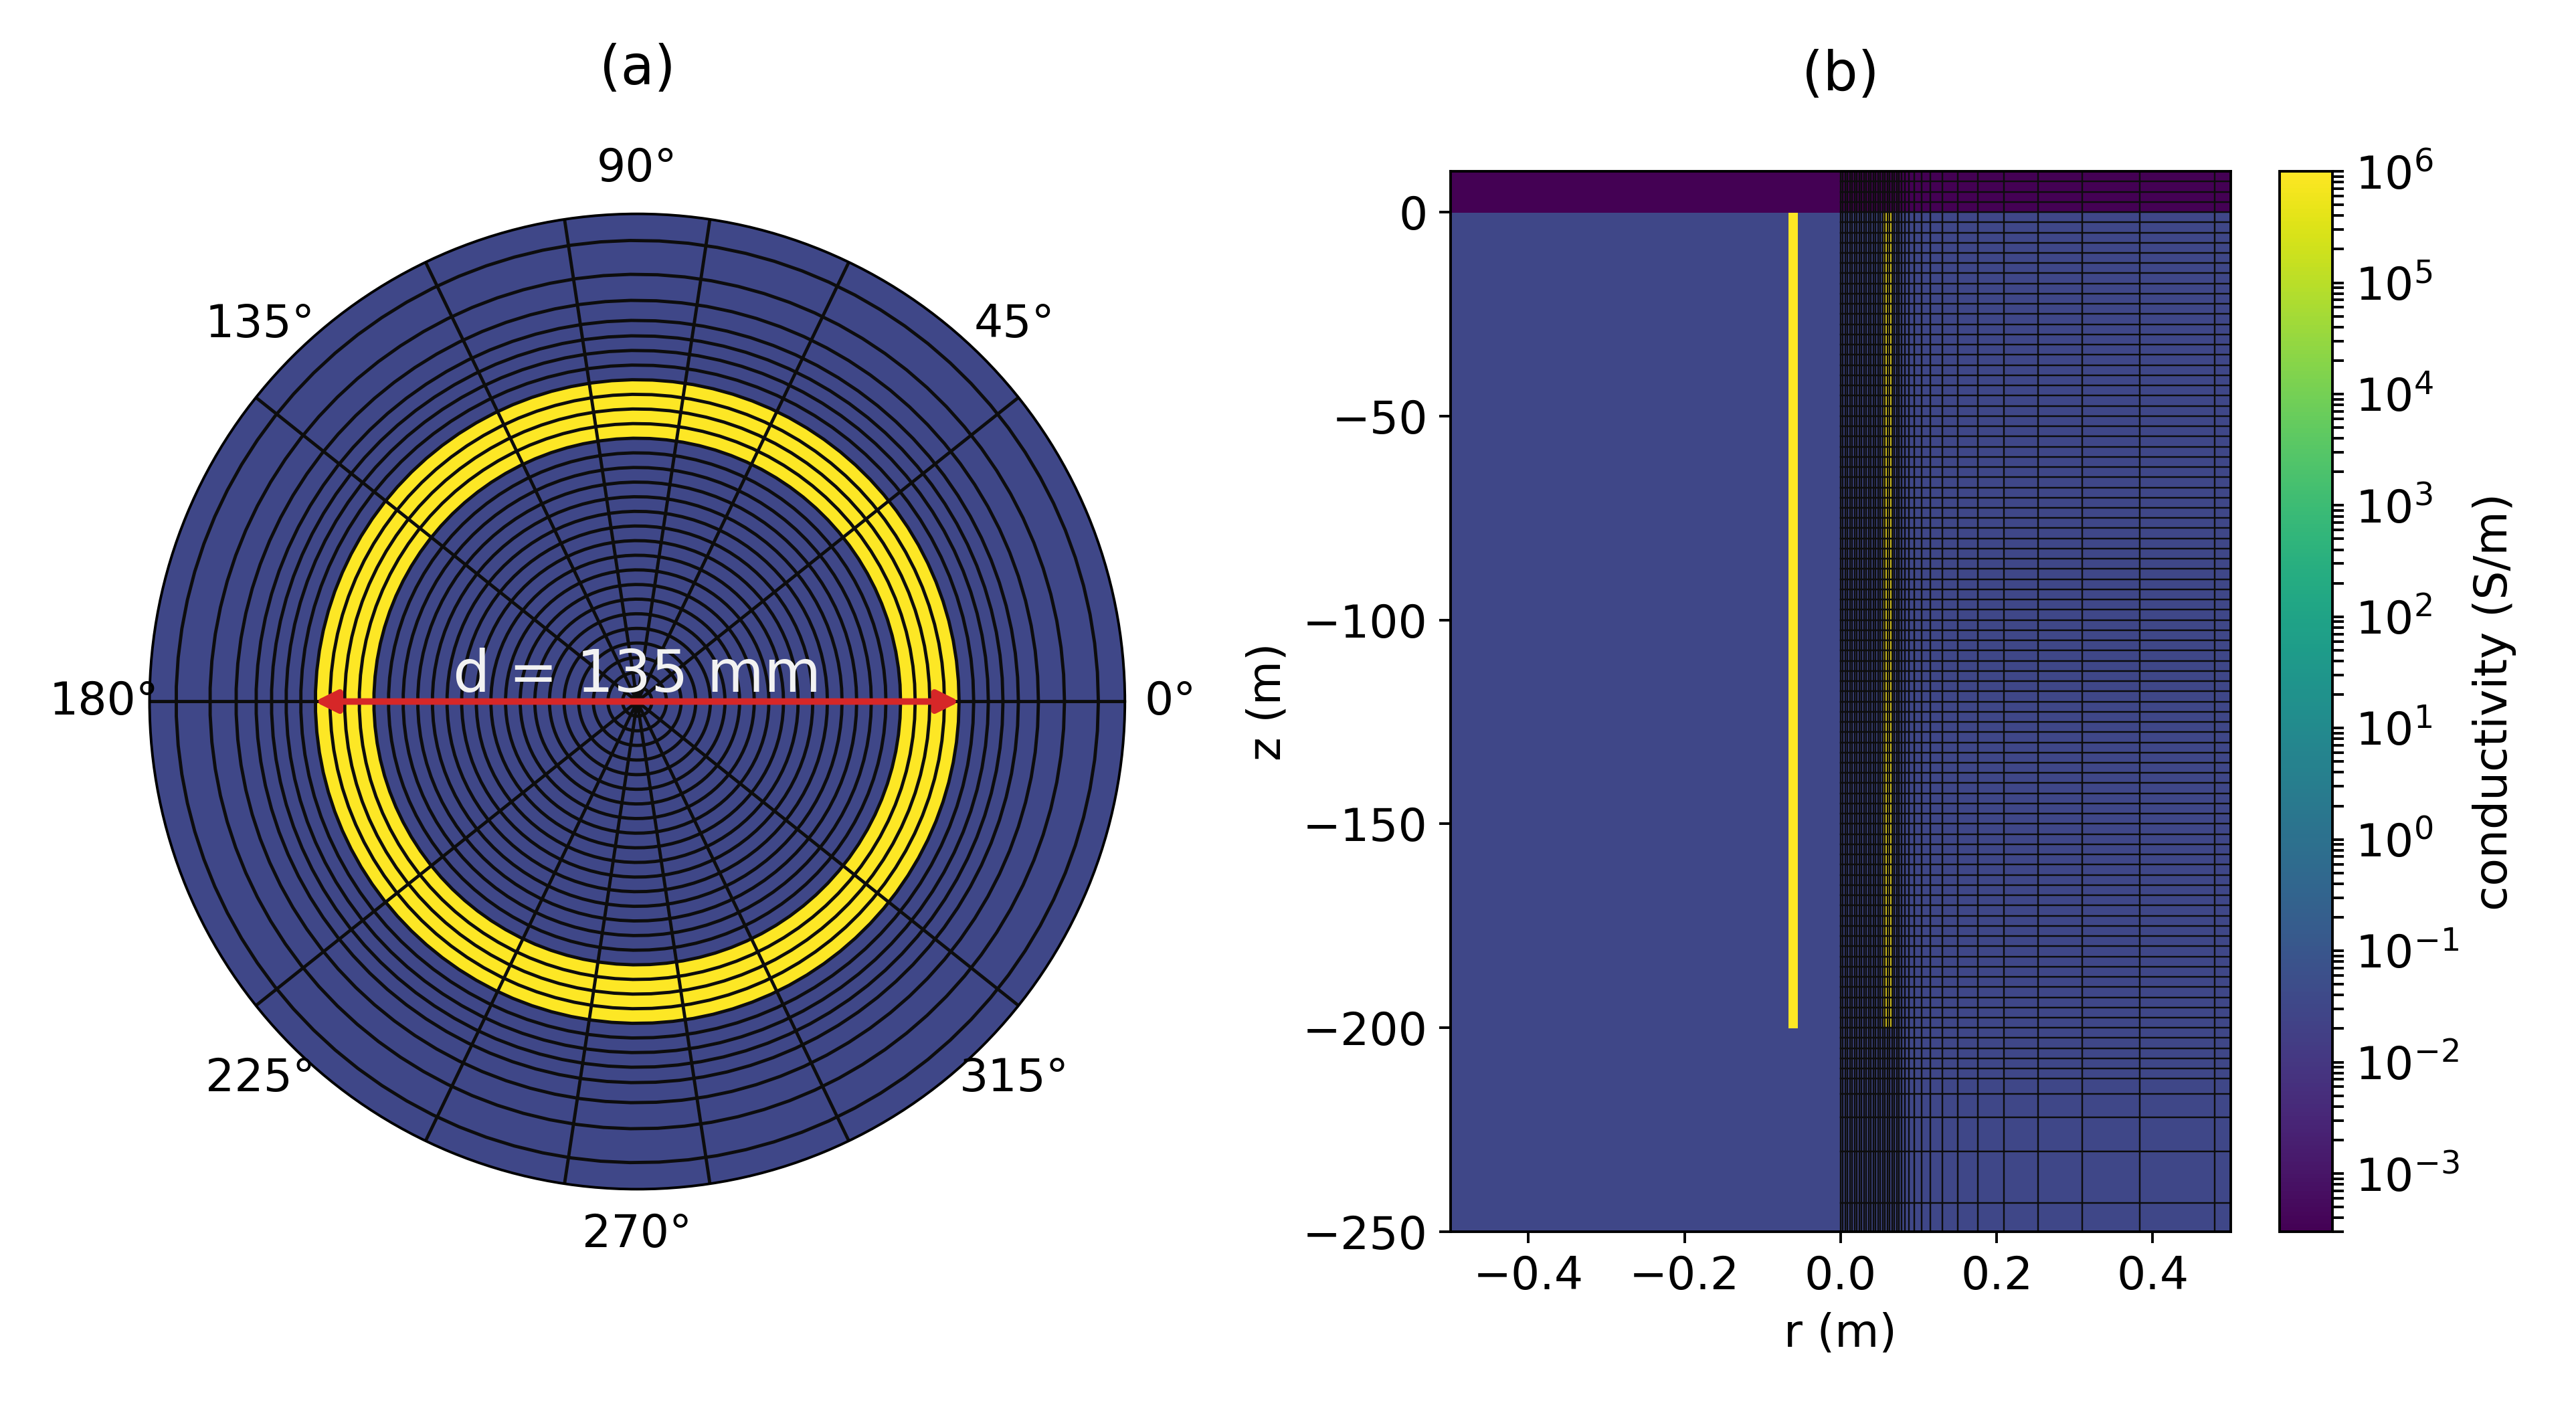
\includegraphics[width=0.8\columnwidth]{figures/casing_software/commer_model.png}
    \end{center}
\caption{
    Depth slice (left) and cross section (right) through the 3D cylindrical
    mesh used for the comparison with \cite{Commer2015}.
    The source and recievers are positioned along the $\theta = 90^\circ$ line.
    The mesh extends 17km raidally and 30km vertically to ensure that the fields
    have sufficiently decayed before reaching the boundaries.
}
\label{fig:commer_model}
\end{figure}



In Figure \ref{fig:commer_results}, I show the absolute value of the radial electric field sampled at five stations; each of the different line colors is associated with a different location, and offsets are with respect to the location of the well. Solutions were interpolated to the same offset using nearest neighbor interpolation.The 3D cylindrical simulation (SimPEG) is plotted with a solid line and overlaps with the UBC solution (dash-dot line) for all times shown. The finite element (FE) solution from \cite{Commer2015} is shown with the dashed lines, and the finite difference (FD) solution is plotted with dotted lines. The 3D cylindrical (SimPEG) and UBC solutions are overall in good agreement with the solutions from \cite{Commer2015}. There is a difference in amplitude and position of the zero-crossing (the v-shape visible in the blue and orange curves) between the Commer solutions and the SimPEG / UBC solutions at the shortest two offsets in the early times. At such short offsets from a highly conductive target, details of the simulation and discretization, such as the construction of the physical property matrices in each of the various approaches become significant; this likely accounts for the discrepancies but a detailed code-comparison is beyond the scope of this chapter. My aim with this comparison is to provide evidence that the numerical simulation is performing as expected; the overall agreement with Commer's and UBC's results is provides confidence that it is.


\begin{figure}[htb]
    \begin{center}
    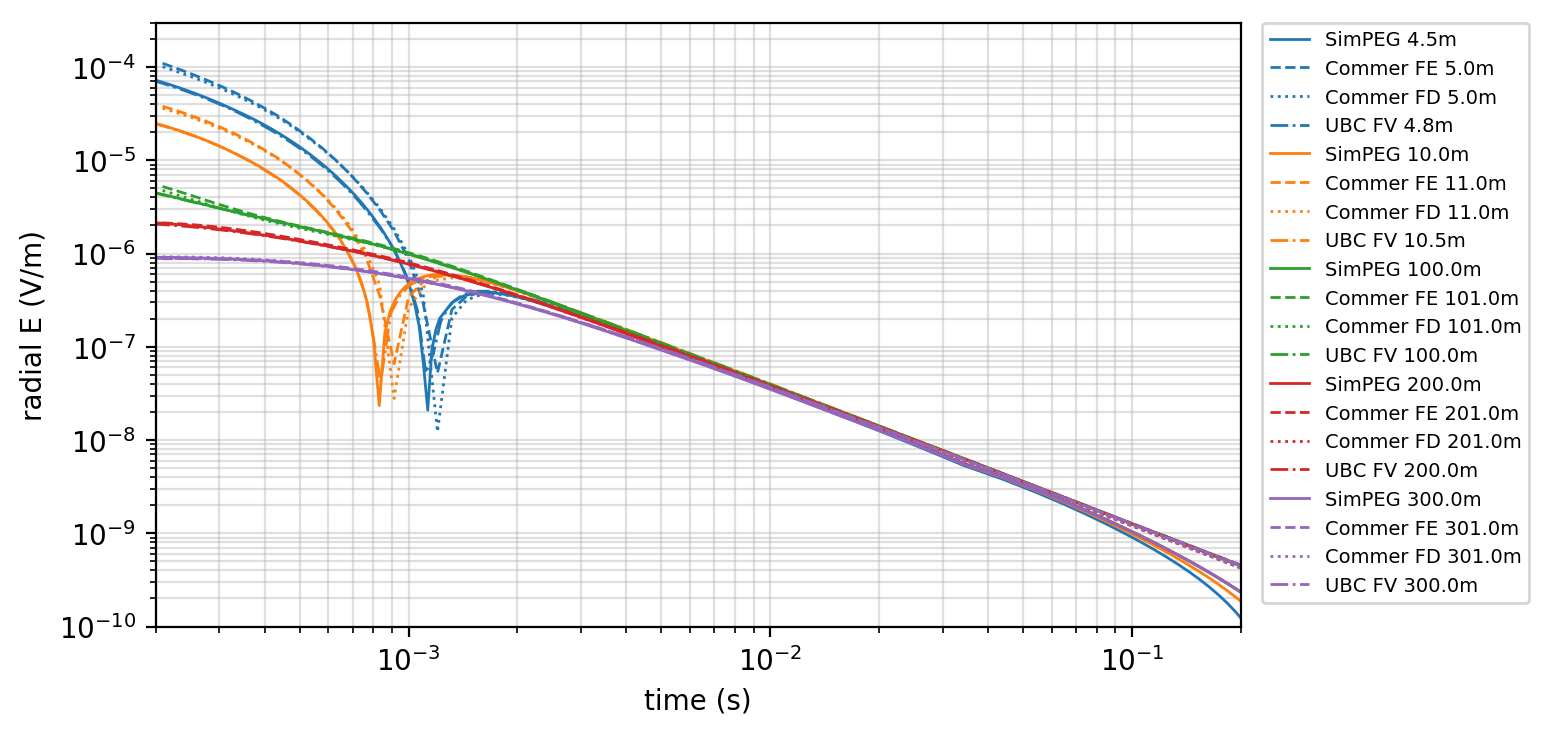
\includegraphics[width=\columnwidth]{figures/commer_results.png}
    \end{center}
\caption{Time domain EM response comparison with \citep{Commer2015}. Each of the different line colors is associated with a different location; offsets are with respect to the location of the well.}
\label{fig:commer_results}
\end{figure}


This example demonstrates agreement between the 3D cylindrical solution and solutions obtained with independently developed codes. Importantly, it also shows how, by using a cylindrical discretization which conforms to the conductivity structure of interest, the size of the mesh and resultant cost of the computation can be greatly reduced. This is true even with relatively conservative spatial and temporal discretizations. Minimizing computation time was not a main focus in the development of the software and there are still opportunities for improving efficiency. As an open-source project, contributions from the wider community are encouraged.
\section{Numerical Examples}
\label{sec:numerical_examples}

The numerical experiments I consider in this section are motivated by the need to use this software to delve into the physics of DC and EM in settings with steel cased wells. As such, the examples build upon examples in analytical derivations and asymptotic analyses in \cite{Kaufman1990, Kaufman1993} at DC and \cite{Augustin1989} for frequency domain EM. I do this to provide confidence that the physical phenomena we observe in the simulations are expected by theory as well as to build a foundation for discussion in the subsequent chapters.
\subsection{DC Resistivity Part 1: Electric fields, currents and charges in a long well}
\label{sec:dc_resistivity_part1}

In his two seminal papers on the topic, Kaufman uses transmission line theory to draw conclusions about the behaviour of the electric field when an electrode is positioned inside of an infinite casing. In this first example, I will revisit some of the physical insights discussed in \citep{Kaufman1990, Kaufman1993} that followed from an analytical derivation and compare those to my numerical results. In the second example, I look at the distribution of current and charges as the length of the well is varied and compare those to the analytical results discussed in \citep{Kaufman1993}

I start by considering a 1 km long well ($10^6$ S/m) in a whole space ($10^{-2}$ S/m), with the conductivity of the material inside the borehole equal to that of the whole space.  For modelling, I will use a cylindrically symmetric mesh. The positive electrode is positioned on the borehole axis in the mid-point of a 1 km long well;  a distant return electrode is positioned 1 km away at the same depth.

Kaufman discusses the behavior of the electric field by dividing the response into three zones: a near zone, an intermediate zone and a far zone \citep{Kaufman1990, Kaufman1993}. In the near zone, the electric field has both radial and vertical components, negative charges are present on the inside of the casing, and positive charges are present on the outside of the casing. The near zone is quite localized and typically, its vertical extent is no more than $\sim 10$ borehole radii away from the electrode. To examine these features in our numerical simulation, I have plotted in Figure \ref{fig:kaufman_zones}: (a)  the total charge, (b) secondary charges, (c) electric field, and (d) current density in a portion of the model near the source.


\begin{figure}
    \begin{center}
    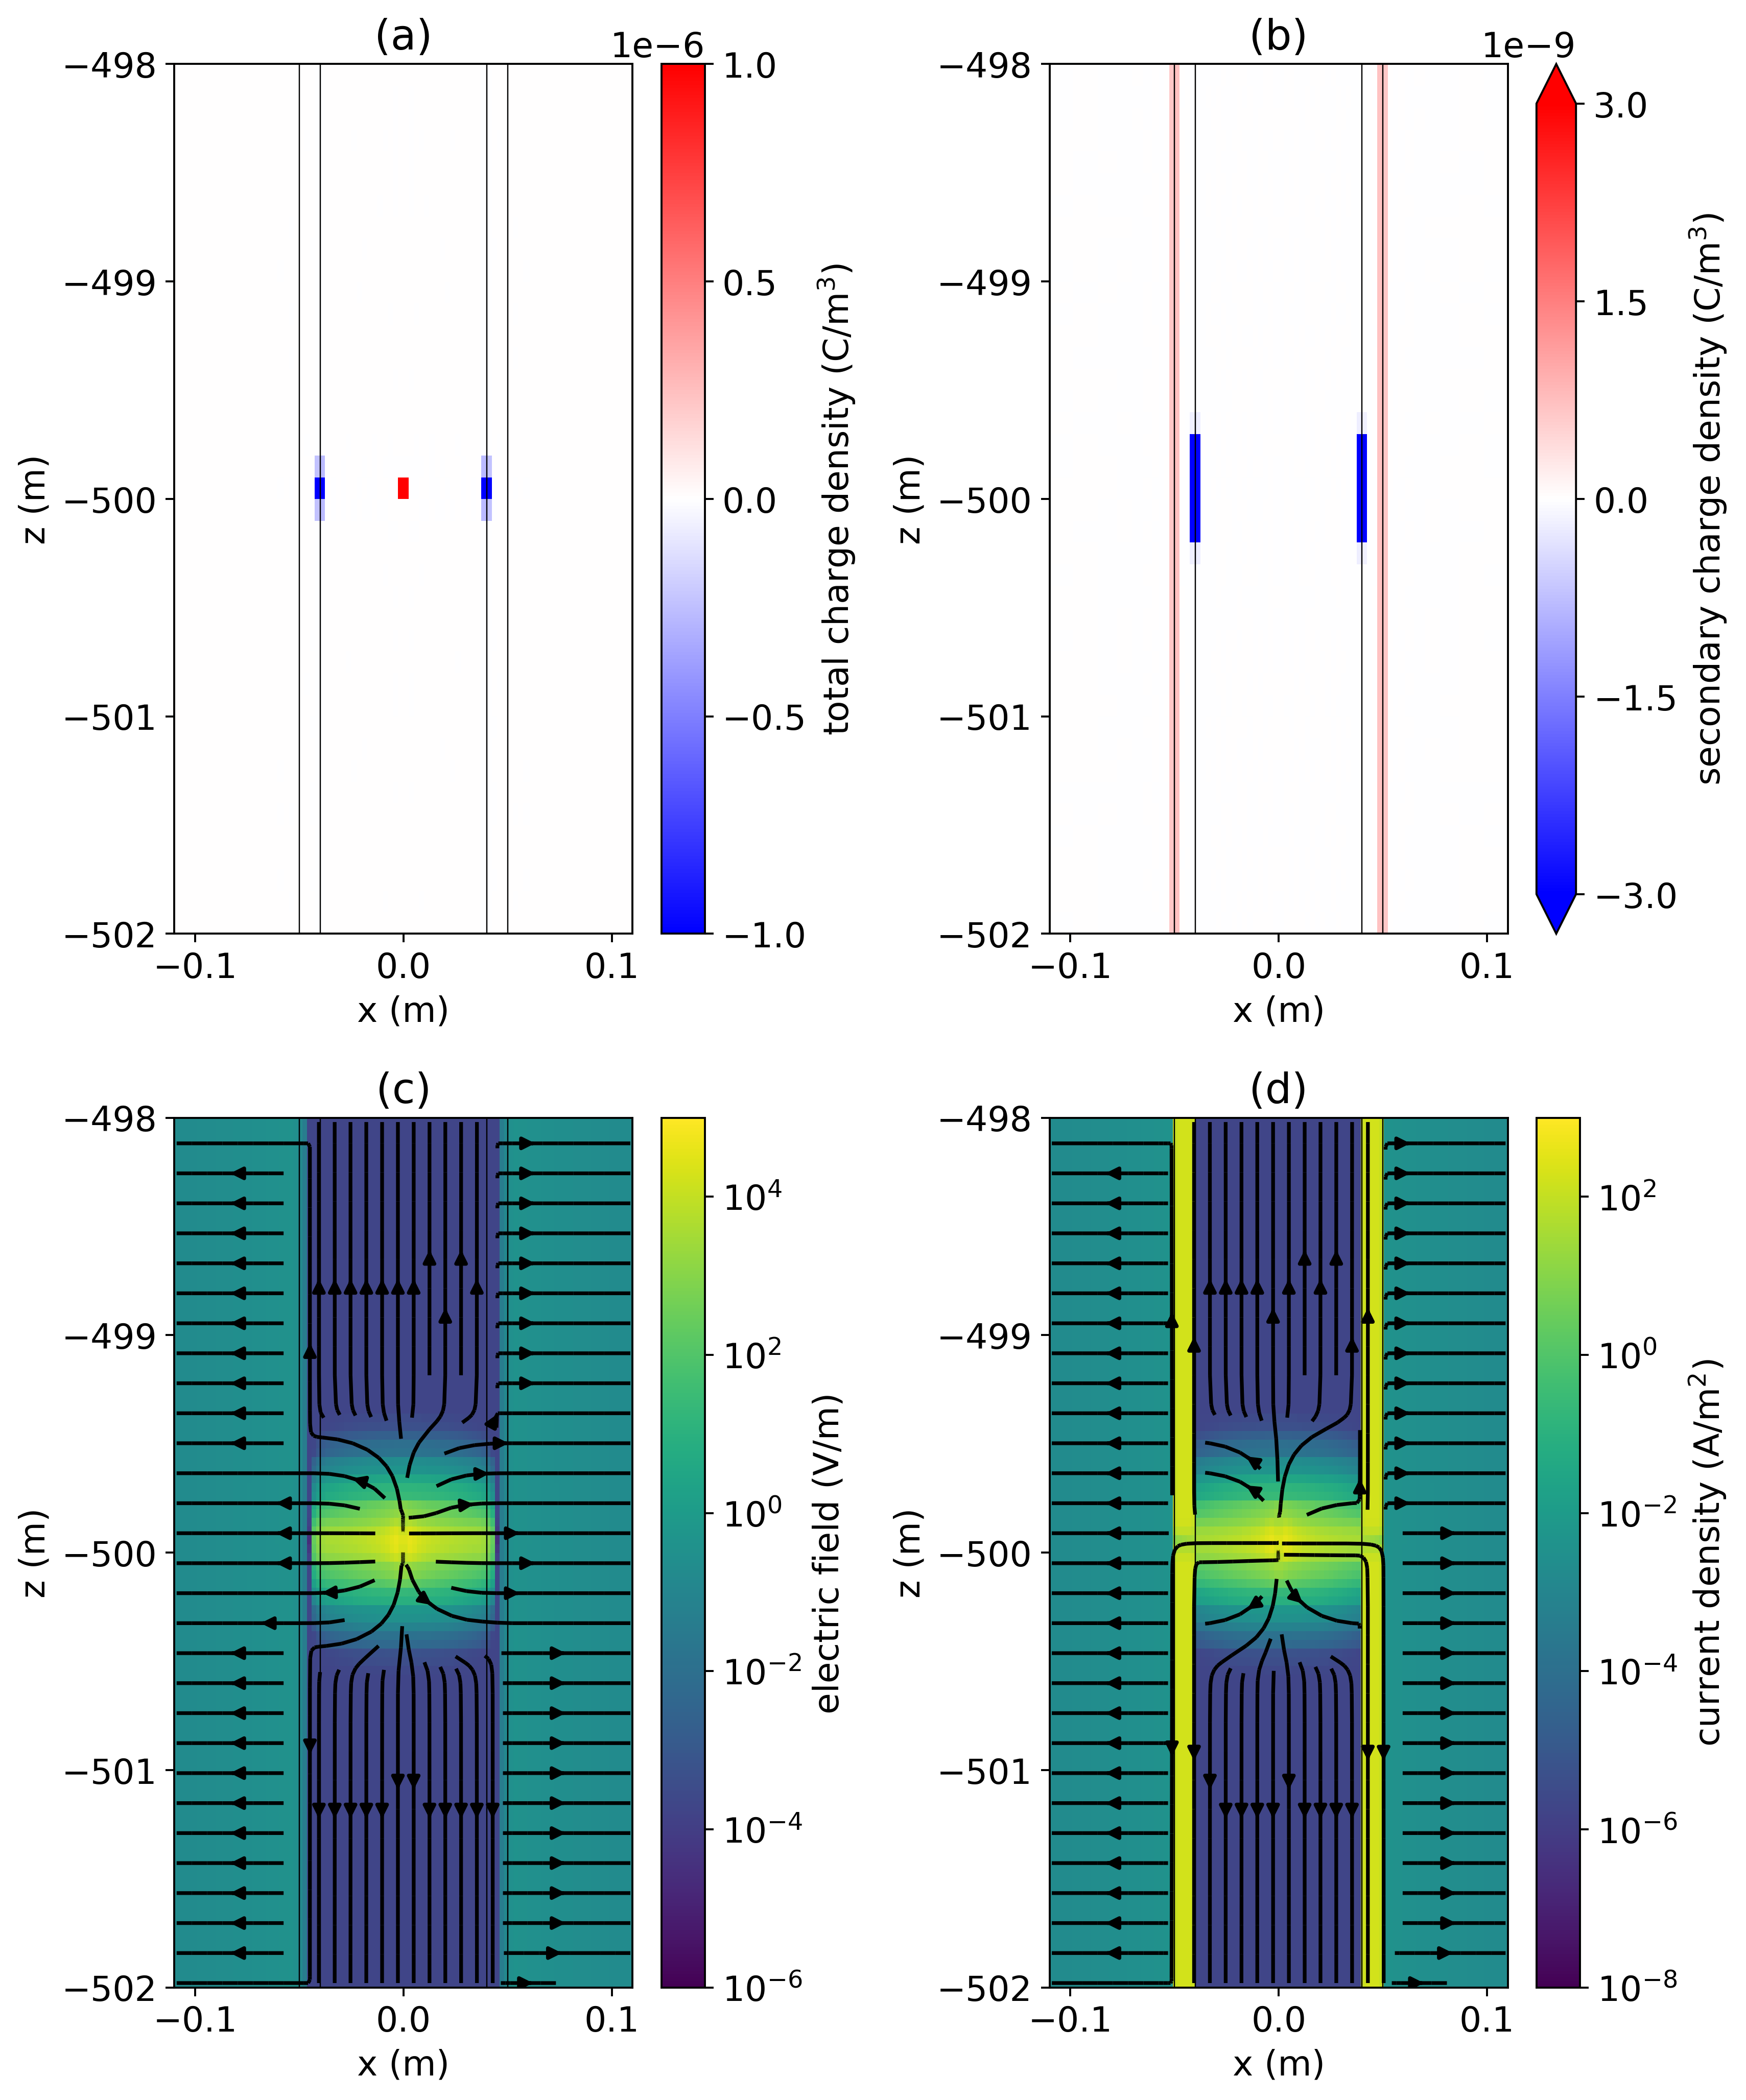
\includegraphics[width=0.7\columnwidth]{figures/casing_software/kaufman_zones.png}
    \end{center}
\caption{(a) Total charge density, (b) secondary charge density, (c) electric field, and (d) current density in a section of the pipe near the source at z=-500m.}
\label{fig:kaufman_zones}
\end{figure}

\subsubsection{Discussion}

Within the near-zone, the total charge is dominated by the large positive charge at the current electrode location and negative charges that exist along the casing wall where current is moving from a resistive region inside the borehole into a conductor. The extent of the negative charges along the inner casing wall is more evident when we look at the secondary charge, which is obtained by subtracting the charge that would be observed in a uniform half-space from the total charge (Figure \ref{fig:kaufman_zones}b). Inside the casing, we can see the transition from near-zone behavior to intermediate zone behavior approximately 0.5 m above and below the source; that is equal to 10 borehole radii from the source location, which agrees with Kaufman's conclusion.

In the intermediate zone, Kaufman discusses a number of interesting aspects with respect to  the behavior of the electric fields and currents which we can compare with the observed behavior in Figure \ref{fig:kaufman_zones}. Among them, he shows that the electric field within the borehole and casing is directed along the vertical axis; as a result no charges accumulate on the inner casing wall. Charges do, however, accumulate on the outer surface of the casing; these  generate radially-directed electric fields and currents, often referred to as “leakage currents”, within the formation. At each depth slice through the casing and borehole, the electric field is uniform, however, due to the high conductivity of the casing, most of the current flows within the casing.  The vertical extent of the intermediate zone depends on the resistivity contrast between the casing and the surrounding formation and extends beyond several hundred meters before transitioning to the far zone, where the influence of the casing disappears \citep{Kaufman1990}.

The radially directed fields from the casing, and the length of the intermediate zone, have practical implications in the context of well-logging because they delineate the region in which measurements can be made to acquire information about the formation resistivity outside the well. Within the intermediate zone, fields behave like those due to a transmission line \citep{Kaufman1990}, and multiple authors have adopted modelling strategies that approximate the well and surrounding medium as a transmission line \citep{Kong2009, Aldridge2015}. I will extend this analysis in the next example and discuss how the length of the well impacts the behavior of the charges, fields, and fluxes.
\subsection{DC Resistivity Part 2: Finite Length Wells}
\label{sec:dc_resistivity_part2}

In \citep{Kaufman1993}, the transmission-line analysis was extended to consider finite-length wells. Inspired by the interest in using the casing as an ``extended electrode'' for delivering current to depth (e.g. \cite{Schenkel1994, Um2015, Weiss2016, hoversten2017borehole}), here I consider a 3D DC resistivity experiment where one electrode is connected to the top of the well. I will examine the current and charge distribution for wells ranging in length from 250 m to 4000 m and compare those to the observations in \citep{Kaufman1993}. The conductivity of the well is selected to be $10^6$ S/m. A uniform background conductivity of $10^{-2}$ S/m is used and the return electrode is positioned 8000 m from the well; this is sufficiently far from the well that we do not need to examine the impact of the return electrode location in this example. A 3D cylindrical mesh was used for the simulation.

\cite{Kaufman1993} derives a solution for the current within a finite length well and discusses two end-member cases: a short well and a long well. ``Short'' versus ``long'' are defined on the product of $\alpha L_c$, where $L_c$ is the length of the casing and $\alpha = 1/\sqrt{S T}$, where $S$ is the cross-sectional conductance of the casing and has units of S$\cdot$m ($S = \sigma_c 2\pi a \Delta a$, for a casing with radius $a$ and thickness $\Delta a$), and $T$ is the transverse resistance. The transverse resistance is approximately equal to the resistivity of the surrounding formation (for more discussion on where this approximation breaks down, see \cite{Schenkel1994}). For short wells, $\alpha L_c \ll 1$, the current decreases linearly with distance, whereas for long wells, where $\alpha L_c \gg 1$, the current decays exponentially with distance from the source, with the rate of decay being controlled by the parameter $\alpha$. In Figure \ref{fig:kaufman_finite_well} (a), I show current in the well for 5 different borehole lengths. The x-axis is the distance from the source normalized by the length of the well. I also show the two end-member solutions (equations 45 and 53) from \cite{Kaufman1993}. There is significant overlap between the 250m numerical solution and the short well approximation. As the length of the well increases, exponential decay of the currents becomes evident. Since $\alpha$ is quite small, for this example $\alpha = 2 \times 10^{-3} ~ m^{-1}$, the borehole must be very long to reach the other end member which corresponds to the exponentially decaying solution.


\begin{figure}[htb]
    \begin{center}
    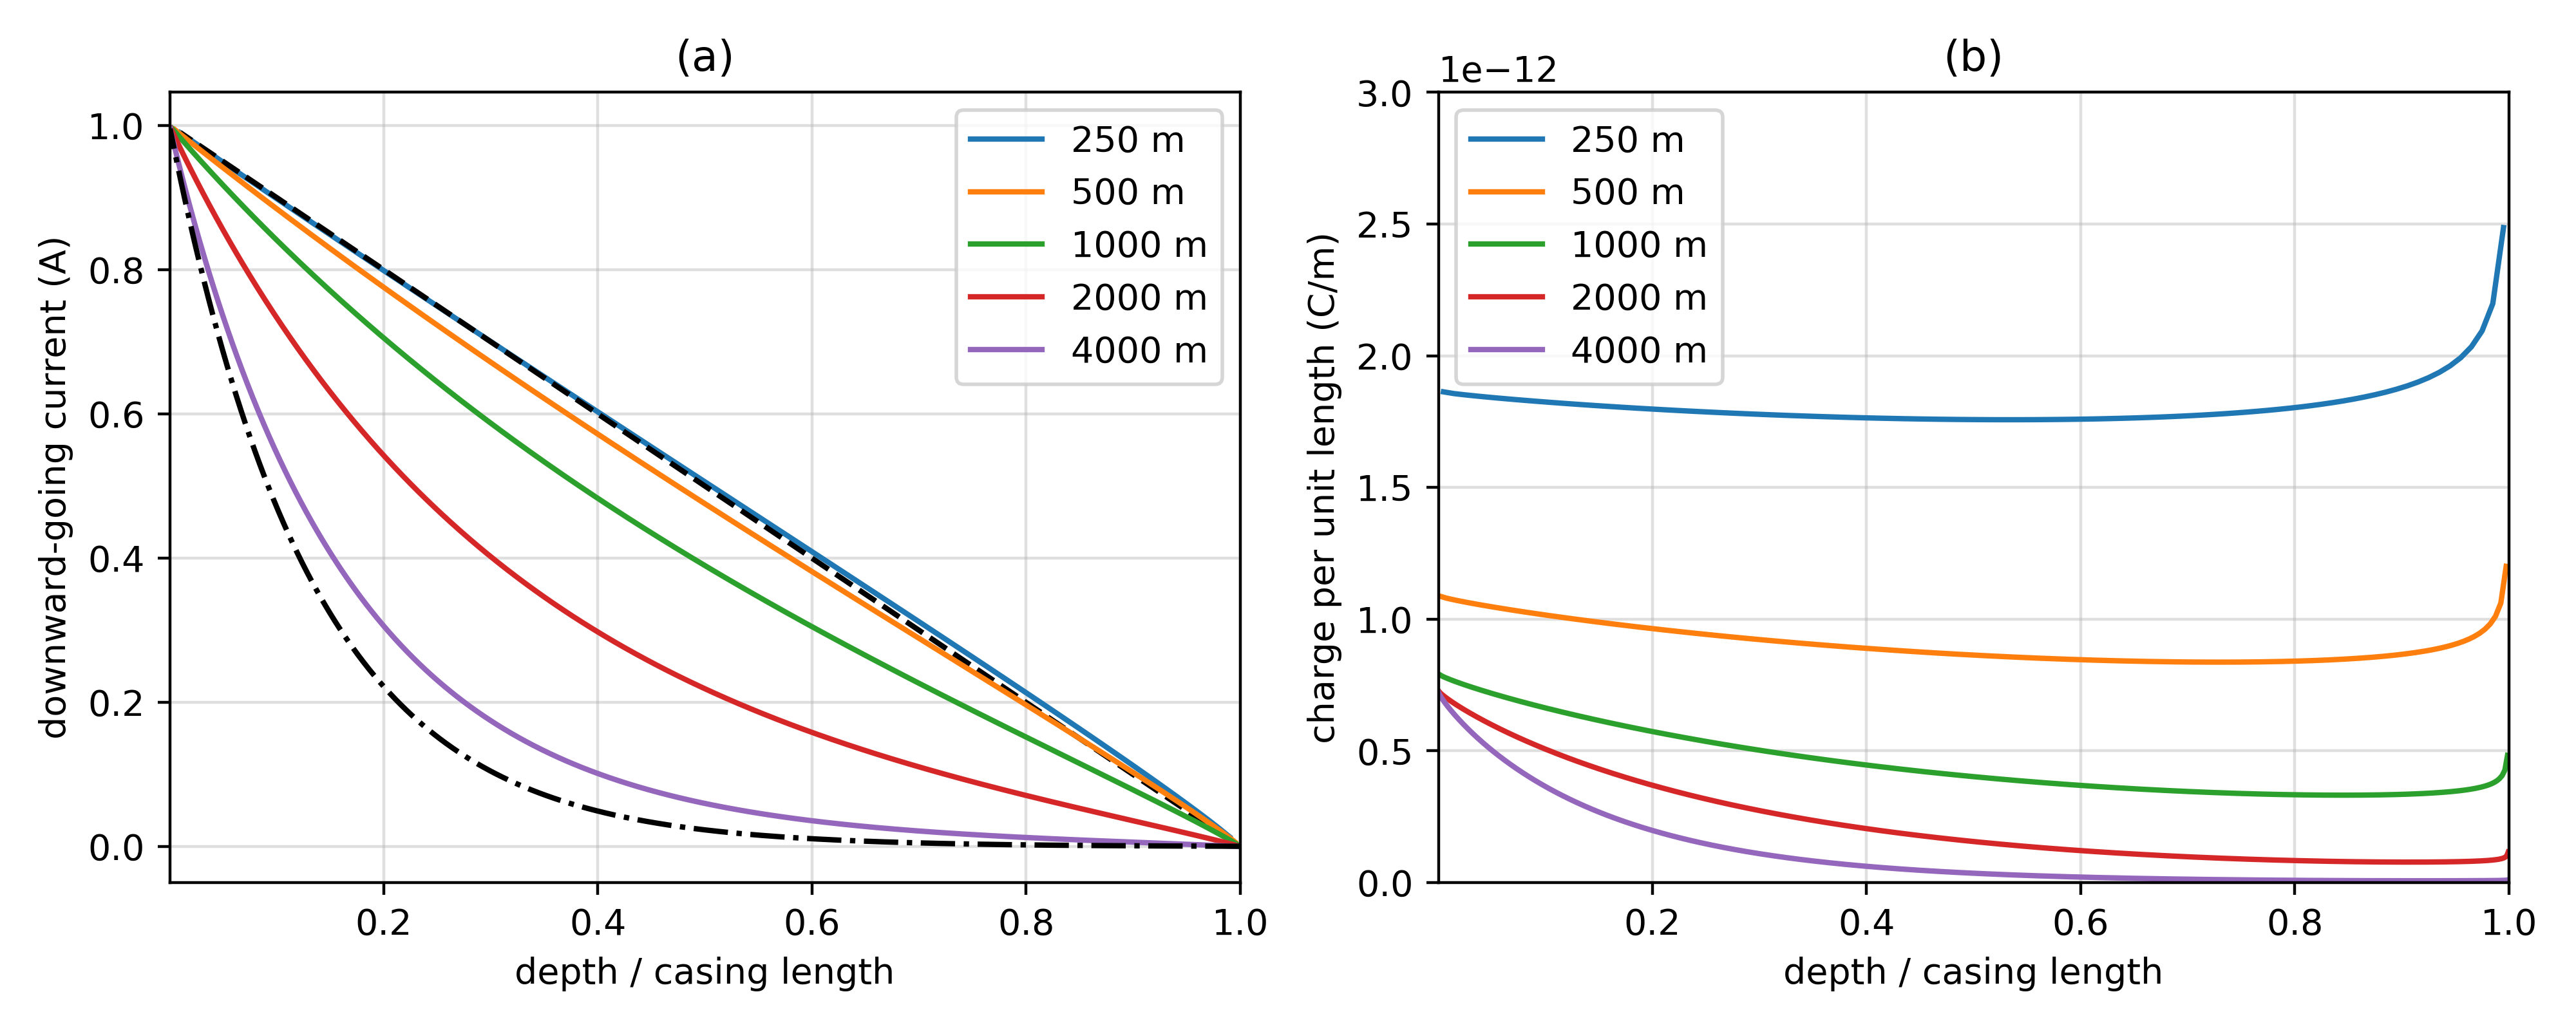
\includegraphics[width=\columnwidth]{figures/kaufman_finite_well.png}
    \end{center}
\caption{
    (a) Current along a well for 5 different wellbore lengths.
    The x-axis is depth normalized by the length of the well. The black
    dashed line shows the short-well approximation (equation 45 in \cite{Kaufman1993})
    for a 200m long well. The black dash-dot line shows the long-well approximation
    (equation 53 in \cite{Kaufman1993}) for a 4000m well.
    (b) Charge per unit length along the well for 5 different wellbore lengths.
}
\label{fig:kaufman_finite_well}
\end{figure}


In Figure \ref{fig:kaufman_finite_well} (b), I have plotted the charges along the length of the well. In the short-well regime, the borehole is approximately an equipotential surface and the charges are uniformly distributed; in the long well the charges decay with depth. What was surprising to me was the noticeable increase in charge accumulation that occurs near the bottom of the well. This is especially evident for the short well. Initially, I was suspicious and thought this might be due to problems with our numerical simulation; there was no obvious physical explanation that I was aware of. However, investigation into the literature revealed that the increase in charge density at the ends of a cylinder is a real physical effect, but an exact theoretical solution does still not appear to exist \citep{Griffiths1997} (see figure 4, in particular).

\subsubsection{Discussion}

The results shown in Figure \ref{fig:kaufman_finite_well} have implications when testing approaches for reducing computational load by approximating a well with a solid tube or prism, as in \cite{Um2015}, or replacing the well with a distribution of charges, as in \cite{Weiss2016}. For a short well, the behaviour of the currents is independent of conductivity, so, as long as the borehole is approximated by a sufficiently conductive target, the behaviour of the fields and fluxes will be representative of the fine-scale model. However, as the length of the well increases, the cross-sectional conductance of the well becomes relevant as it controls the rate of decay of the currents in the well and thus the rate that currents leak into the formation. A similar result holds when a line of charges is used to approximate the well as a DC source; a uniform charge is suitable for a sufficiently short or sufficiently conductive well, whereas a distribution of charge which decays exponentially with depth needs to be considered for longer wells. Thus, when attempting to replace a fine-scale model of a well with a coarse-scale model, either with a conductivity structure or by some form of ``equivalent source'', validations should be performed on models that have the same length-scale as the experiment to ensure that both behaviors are being accurately modeled.

\subsection{Frequency Domain Electromagnetics Part 1: Comparison with scale model results}
\label{sec:FDEM_part1}

In the DC example, we discussed how charges are distributed along the well and currents flow into the formation. From a historical perspective, practical developments in EM were pursued in the frequency domain; the mathematics is more manageable in the frequency domain, and technological advances were being made in the development of induction well-logging tools \citep{Doll1949, Moran1962}. Although the conductivity of the pipes generally plays the most dominant role in attenuating the signal, the magnetic permeability is non-negligible \citep{Wait1977}; it is the product of the conductivity and permeability that appears in the description of EM attenuation. Also, the fact that permeable material becomes magnetized in the presence of an external field complicates the problem.
\cite{Augustin1989} is one of the first papers on induction logging in the presence of steel cased wells that aims to understand and isolate the EM response of the steel cased well. Using a combination of scale modelling and analytical mathematical modelling, they examine the impacts of conductivity and magnetic permeability on the magnetic field observed in the pipe. In this example and the one that follows, I attempt to unravel this interplay between conductivity and magnetic permeability.

The first experiment \cite{Augustin1989} discusses is a scale model using two different pipes, a conductive copper pipe and a conductive, permeable iron pipe; each pipe is 9 m in length. The copper pipe had an inner diameter of 0.063 m and a thickness of 0.002 m, while the iron pipe had a 0.063 m inner diameter and 0.0043 m wall thickness. A source-loop, with radius 0.6 m was co-axial with the pipe and in one experiment positioned at one end of the pipe (which they refer to as the ``semi-infinite pipe'' scenario). In another experiment the source loop is positioned at the midpoint of the pipe (which they refer to as the ``infinite pipe'' scenario); for both experiments, magnetic field data are measured as a function of frequency at the central axis of the pipe. Their results are presented in terms of a Field Strength Ratio (FSR), which is the ratio of the absolute value of the magnetic field at the receiver with the absolute value of the magnetic field if no pipe is present (Figure 3 in \cite{Augustin1989}). At low frequencies, for the data collected within the iron pipe, static shielding (FSR $<$ 1) was observed for the measurements where the receiver was in the plane of the source loop for both the ``infinite'' and ``semi-infinite'' scenarios. When the receiver was positioned within the pipe, 1.49 m offset from the plane of the source loop, static enhancement effects (FSR $>$ 1) were observed for both the infinite and semi-infinite scenarios. Using this experiment for context, I will compare the behaviour of our numerical simulation with the observations in \citep{Augustin1989} and examine the nature of the static shielding and enhancement effects.

For our numerical setup, the pipes are 9 m in length and have an inner diameter of 0.06 m. The copper pipe has a casing-wall thickness of 0.002 m and the iron pipe has a thickness of 0.004 m. Following the estimated physical property values from \cite{Augustin1989}, I use a conductivity of $3.5 \times 10^7$ S/m and a relative permeability of 1 for the copper pipe. For the iron pipe, a conductivity of $8.0 \times 10^6$ S/m and a relative permeability of 150 is used. A background resistivity of $10^4 ~\Omega$m is assumed. The computed FSR values for the axial magnetic field as a function of frequency are shown in Figure \ref{fig:AugustinFSR}.


\begin{figure}
    \begin{center}
    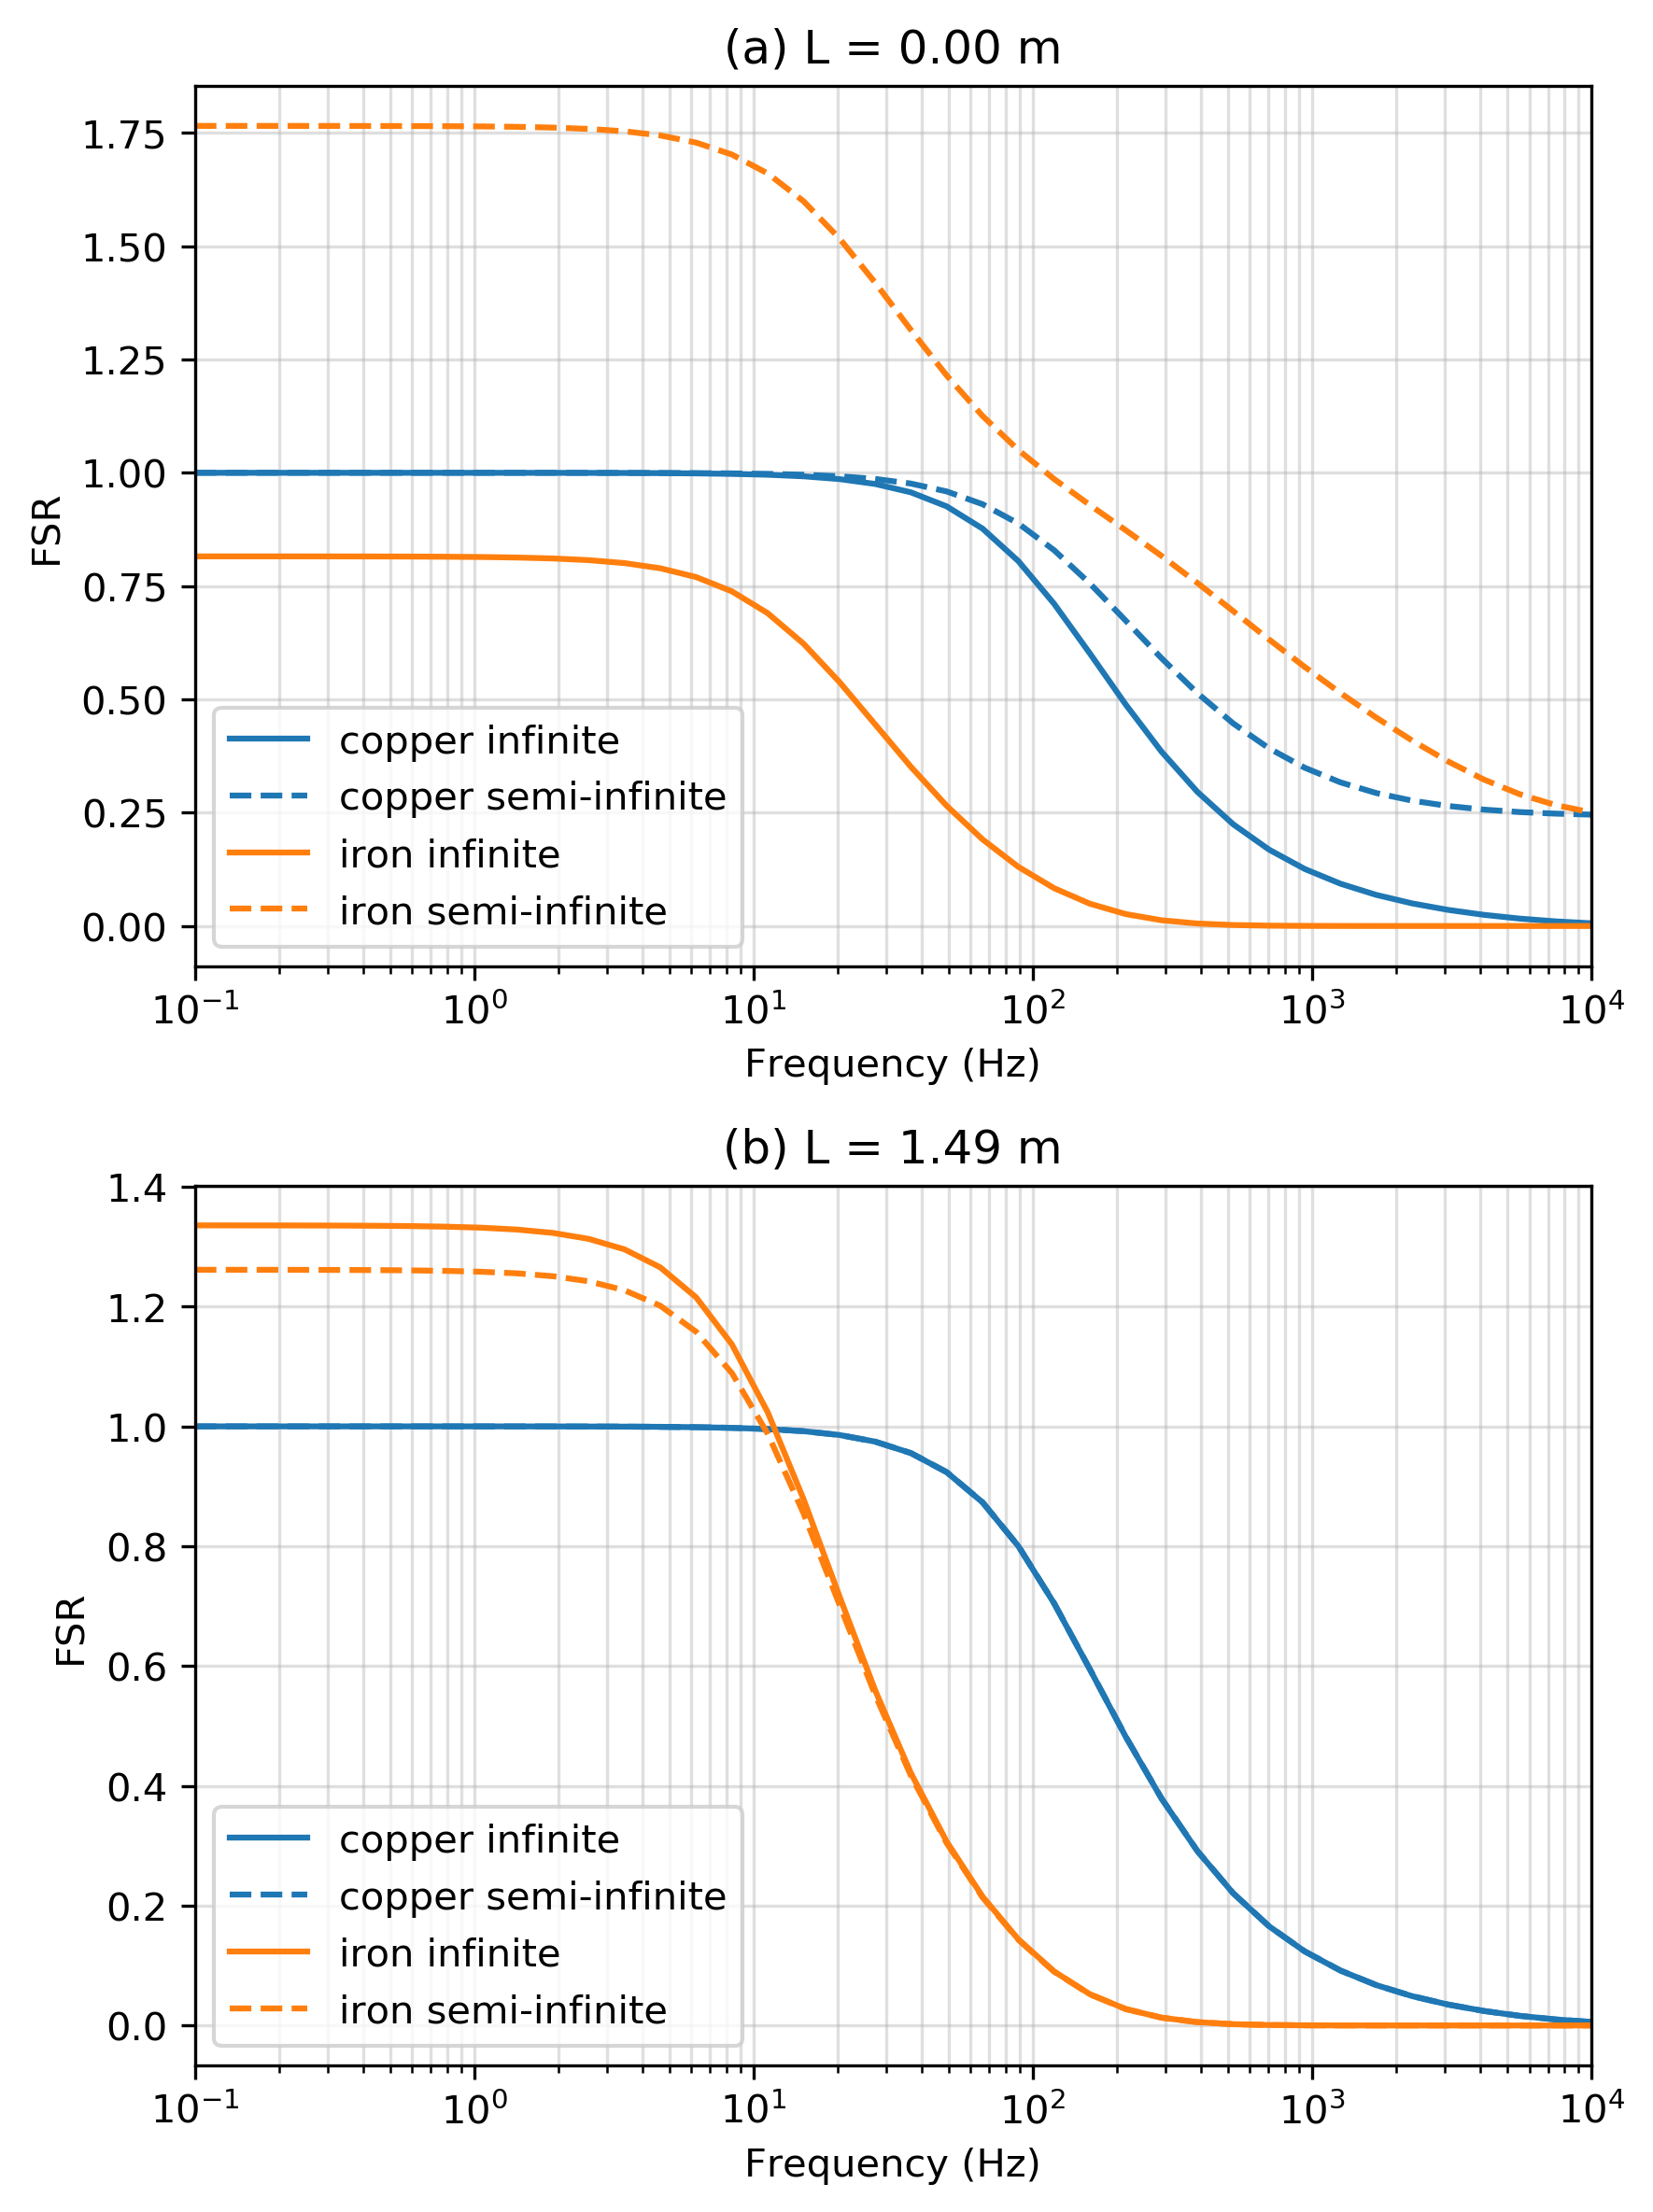
\includegraphics[width=0.6\columnwidth]{figures/casing_software/AugustinFSR.png}
    \end{center}
\caption{
    Field strength ratio (FSR), the ratio of the measured vertical magnetic field with the free space magnetic field, as a function of frequency for two different reciever locations.
    In (a), the reciever is in the same plane as the source, in (b), the reciever is 1.49m offset from the source.
}
\label{fig:AugustinFSR}
\end{figure}


Consider the response of the conductive pipe. At low frequencies, the FSR for the copper pipe (blue lines) is 1 for both the infinite (solid line) and semi-infinite (dashed line) scenarios, as the field inside the copper pipe is equivalent to the free-space field. With increasing frequency, eddy currents are induced in the pipe which generate a magnetic field that opposes the primary, causing a decrease in the observed FSR. When the source and receiver are in the same plane (L=0.00 m), the rate of decrease is more rapid in the infinite scenario than the semi-infinite. Since there is conductive material on both sides of the receiver in the infinite case, we would expect attenuation of the fields to occur more rapidly than in the semi-infinite case. This observation is consistent with Figure 3a in \cite{Augustin1989}. For the offset receiver (L=1.49 m), they observed a slight separation in the infinite and semi-infinite curves which I do not; however, they attributed this to potential errors in magnetometer position. Thus, overall, the numerical results for the copper pipe are in good agreement with the scale model results observed by \cite{Augustin1989}.

Next, we examine the response of the conductive, permeable pipe. In Figure \ref{fig:AugustinFSR}b, we observe a static enhancement effect (FSR $>$ 1) at low frequencies. The enhancement is larger in the infinite scenario than the semi-infinite scenario; this is in agreement with Figure 3b in \cite{Augustin1989}. There is however, a significant discrepancy between our numerical simulations and the scale model for the semi-infinite pipe when the source and receiver lie in the same plane(Figure \ref{fig:AugustinFSR}a). \cite{Augustin1989} observed a static shielding effect for both the infinite and semi-infinite scenarios, whereas we observe a static shielding for the infinite scenario, but a significant static enhancement for the semi-infinite case. To examine what might be the cause of this, I will examine the magnetic flux density in this region of the pipe.

In Figure \ref{fig:AugustinBfields}, I have plotted: (a) the secondary magnetic flux in the infinite-pipe scenario near the source ($z=$-4.5 m), (b) the secondary magnetic flux in the semi-infinite scenario (z=0 m for the source), and (c) top 5 cm of the semi-infinite pipe. All plots are at 0.1 Hz. The primary magnetic field is directed upwards within the regions I have plotted, so upward-going magnetic flux indicates a static enhancement effect, and downward-oriented magnetic flux indicates static shielding effects. In (a) we see a transition between the static shielding in the vicinity of the source to a static enhancement approximately 0.5 m above and below the plane of the source. Similarly in (b), we notice a sign-reversal in the z-component of the secondary magnetic flux at a depth of 0.6 m.

\subsubsection{Discussion}
The behaviors observed in Figure \ref{fig:AugustinBfields} are quite comparable to Augustin et al.'s observation of a transition from shielding to enhancement occurring at distances greater than 0.8 m from the source. Numerical experiments show that the vertical extent of the region over which static shielding is occurring increases with increasing pipe diameter, and similarly increases with increasing loop radius while the magnitude of the effect decreases. This can be understood by considering how the pipe is magnetized; for a small loop radius, the magnetization is largely localized near the plane of the source and rapidly falls off with distance from the plane of the source. Localized, large amplitude magnetization causes the casing to act as a collection of dipoles around the circumference of the casing. As the radius of the loop increases, the magnetization spreads out along the length of the well resulting in longer, lower-amplitude dipoles, thus both increasing the extent of the region over which static shielding is occurring as well as decreasing its amplitude.


\begin{figure}
    \begin{center}
    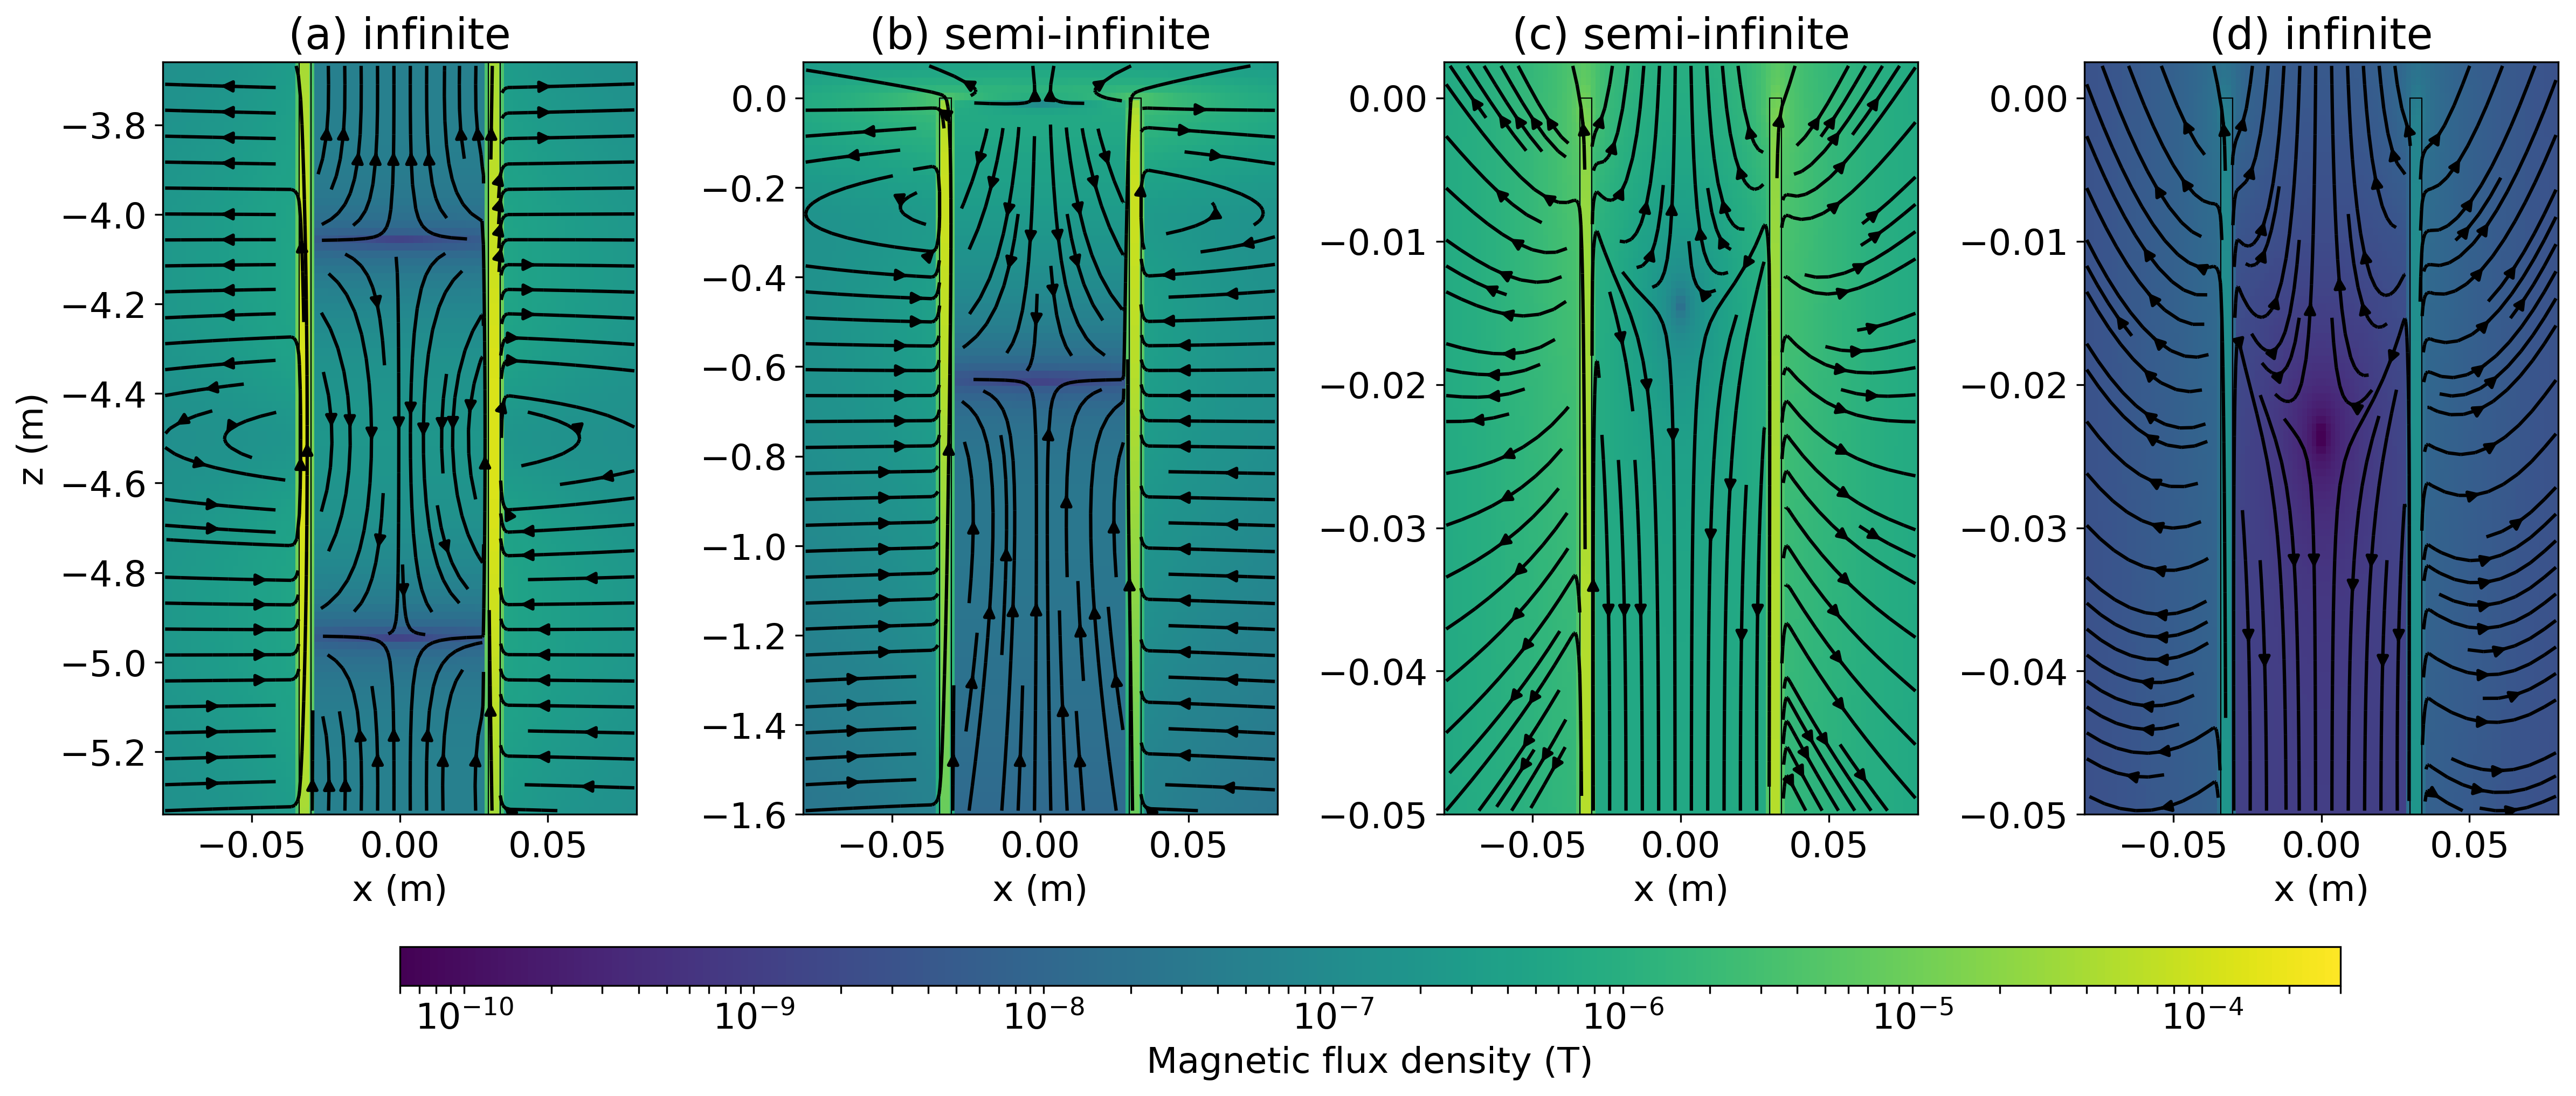
\includegraphics[width=\columnwidth]{figures/casing_software/AugustinBfields.png}
    \end{center}
\caption{
    Magnetic flux density at 0.1 Hz in the region of the pipe near the plane of the source for
    (a) the ``infinite'' pipe, where the source is located at -4.5 m and the pipe extends from 0 m to -9 m,
    (b) a ``semi-infinite'' pipe, where the source is located at 0 m and the pipe extends to -9 m.
    In (c), we zoom in to the top 5 cm of the ``semi-infinite'' pipe,
    and (d) shows the 5 cm at the top-end of the ``infinite'' pipe.
}
\label{fig:AugustinBfields}
\end{figure}


This explains the nature of the static enhancement and static shielding effects, but to explain the discrepancy between the static shielding observed in the semi-infinite pipe when L=0 m by Augustin et al., and the static enhancement we observe in Figure \ref{fig:AugustinFSR}a, I examine the magnetic flux density in the top few centimeters of the pipe. Figure \ref{fig:AugustinBfields}c shows the top 5 cm of the secondary magnetic flux in the semi-infinite pipe; the source is in the z=0 m plane.  Zooming in reveals there is yet another sign reversal near the end of the pipe. This is evident even in the infinite-pipe scenario (Figure \ref{fig:AugustinFSR}d), where the source is offset by several meters from the end of the pipe. This edge-effect perhaps bears some similarities to what we observed in Figure \ref{fig:kaufman_finite_well}b, where we saw a build up of charge near the end of the pipe in the DC scenario. At the end of the pipe, we encounter the situation where the normal component of the flux ($\vec{j}, \vec{b}$) from the pipe to the background needs to be continuous both in the radial and vertical directions at the end of the pipe as does the tangential component of the fields ($\vec{e}, \vec{h}$). The interplay of these two constraints at the end of the pipe results in more complexity in the resultant fields and fluxes. Within the span of a few centimeters we transition from static enhancement at the top of the pipe to a static shielding further down. An error as small as a few centimeters in the position of the magnetometer causes a reversal in behavior; in Figure \ref{fig:Augustin3cm}, I have plotted the FSR for a magnetometer positioned 3 cm beneath the plane of the source, and the static-shielding behavior observed for the semi-infinite pipe is much more aligned with that observed in Figure 3a in \cite{Augustin1989}.



\begin{figure}
    \begin{center}
    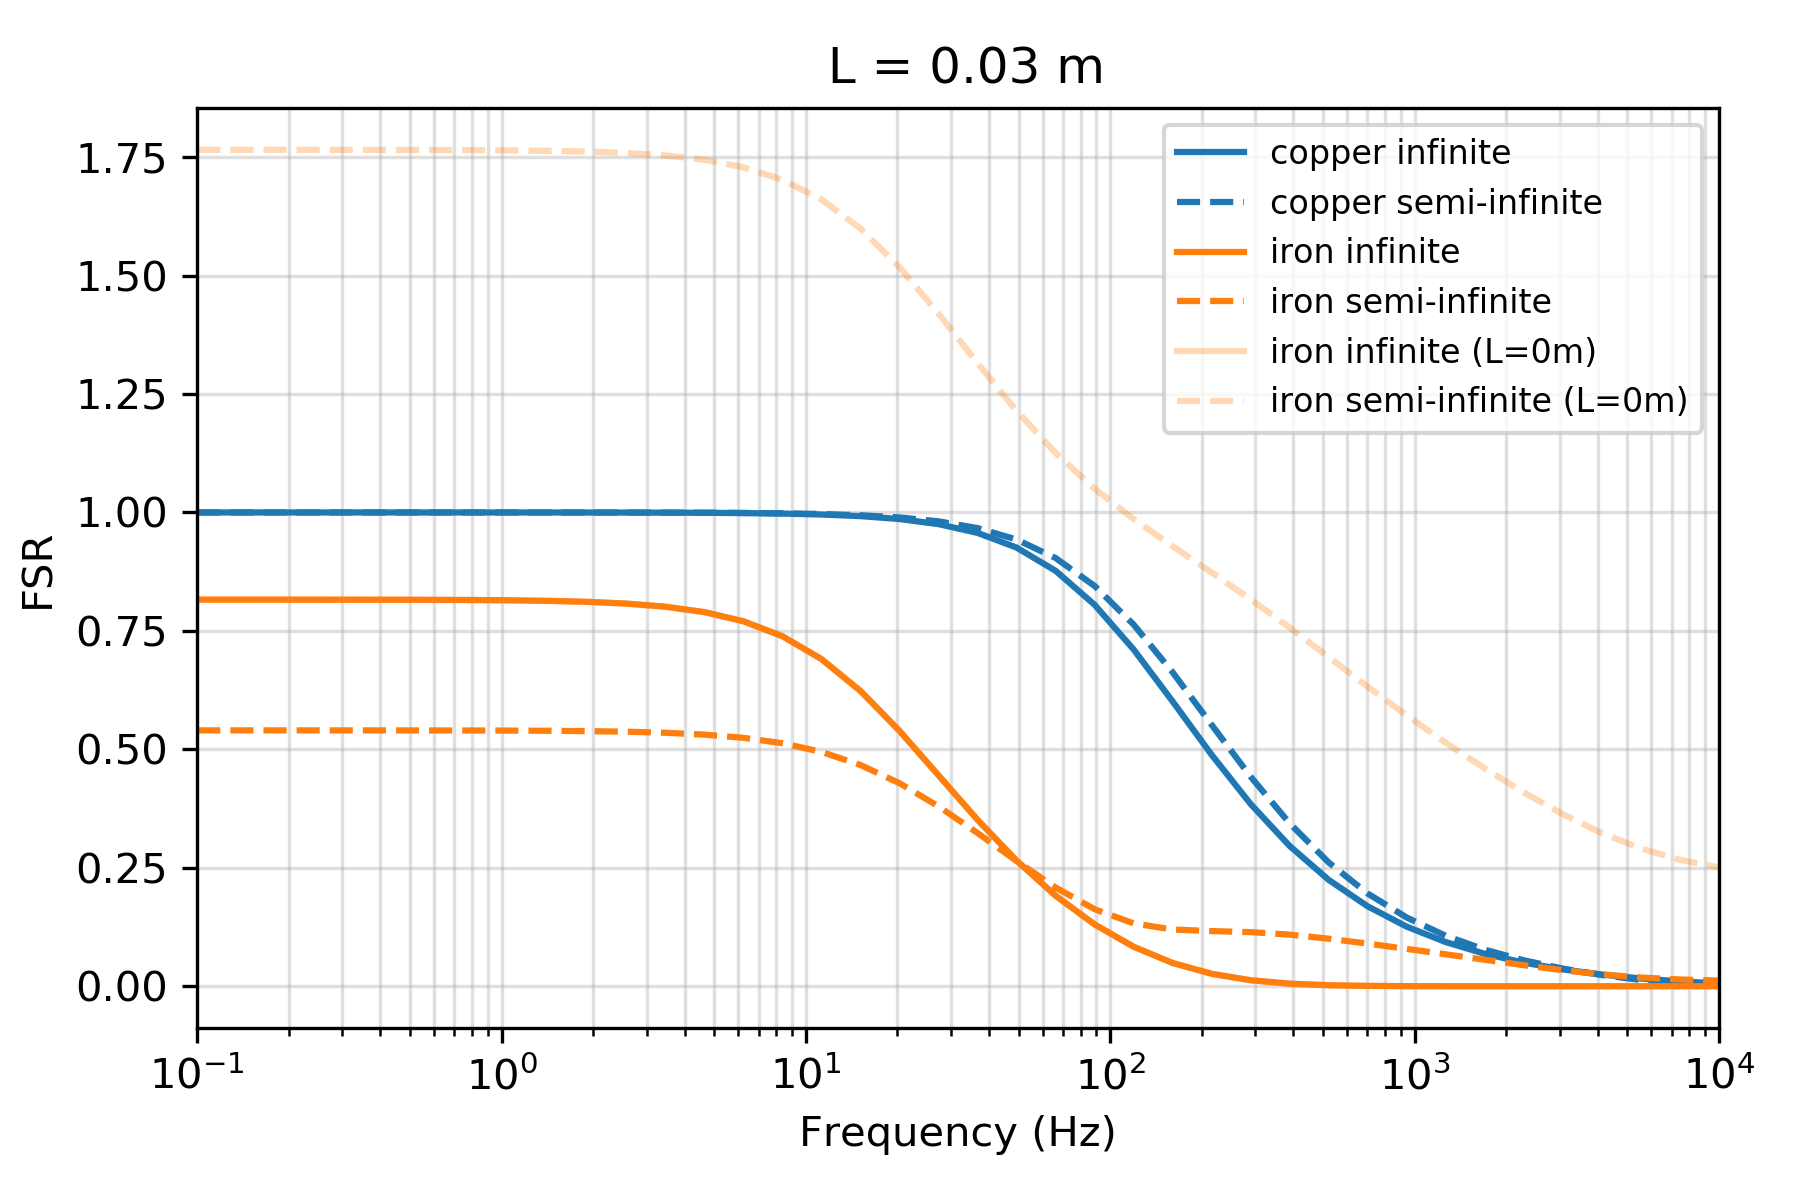
\includegraphics[width=0.6\columnwidth]{figures/Augustin3cm.png}
    \end{center}
\caption{
    Field strength ratio, FSR, for a reciever positioned 3cm beneath
    the plane of the source. For comparison, we have plotted the
    FSR for the permeable pipe when the source and reciever lie in the same
    plane (L=0.00m) with the semi-transparent orange lines.
    Note that the infinite-pipe solutions for L=0.03m and L=0.00m overlap.
}
\label{fig:Augustin3cm}
\end{figure}





\subsection{Frequency Domain Electromagnetics Part 2: Conductivity and permeability in the inductive response of a well}
\label{sec:FDEM_part2}

The experiments shown in the previous section revealed some insights into the complexity of the fields within the pipe and illustrated the role of permeability in the character of the responses at low frequency. Next, we move to larger scales and examine the role of conductivity and permeability in the responses we observe in the borehole.

In this example, I consider a 2 km long well with an outer diameter of 10 cm and thickness of 1 cm in a whole-space which has a resistivity of $10^4$ $\Omega$m. A loop with radius 100 m is coaxial with the well and positioned at the top-end of the well. A receiver measuring the z-component of the magnetic flux density is positioned 500 m below the transmitter loop, along the axis of the well. I will consider both time domain and frequency domain responses.

In electromagnetics, it is often the product of permeability and conductivity that is considered to be the main controlling factor on the EM responses. To assess the contribution of each to the measured responses, I will investigate two scenarios. In the first, the well has a conductivity of $10^8$ S/m and a relative permeability of 1, and in the second, the well has a conductivity of $10^6$ S/m and a relative permeability of 100; thus the product of conductivity and permeability is equivalent for both wells.

Similar to the analysis done by \cite{Augustin1989} when looking at the role of borehole radius in the behaviour of the magnetic response (e.g. figure 8), I will examine the normalized secondary field (NSF) which is the ratio of the secondary field with the amplitude of the primary, where the primary is defined to be the free-space response. In Figure \ref{fig:fdemNSF}, I have plotted the normalized secondary field for the two pipes considered, the conductive pipe (blue) and the conductive, permeable pipe (orange). Let us start by examining the conductivity response in Figure \ref{fig:fdemNSF}. Where the value of the NSF is zero, the primary dominates the response; this is the case at low frequencies where induction is not yet contributing to the response. As frequency increases, currents are induced in the pipe which generate a secondary magnetic field that opposes the primary, hence the NSF becomes negative. When the real part of the NSF (solid line) is -1, the secondary magnetic field is equal in magnitude but opposite in direction to the free-space primary and the measured real field is zero. Values less than -1 indicate a sign reversal in the real magnetic field. Similarly, when the imaginary part of the response function goes above zero, there is a sign reversal in the imaginary component. Note that these sign reversals occur even in a half-space and are a result of sampling the fields within a conductive medium; in this case the receiver was 500 m below the surface.

As compared to the conductive pipe, the frequency at which induction sets in is higher for the conductive, permeable pipe. We also notice that the amplitude variation of both the imaginary and real parts is larger for the permeable pipe. To examine the contribution of conductivity and permeability to the responses, I have plotted the real part of the secondary magnetic flux density, $\mathbf{b}$, in Figure \ref{fig:bfdem}. The top row shows the response within the conductive pipe and the bottom row shows the conductive, permeable pipe. The primary magnetic flux is oriented upwards and we can see that all of the secondary fields generated are oriented downwards. Similar to the previous example, we see that at low frequencies, there is magnetostatic response due to the permeable pipe. However, due to the larger length scales of the source loop and the casing in this example, there is no measurable contribution at the receiver. At 1 Hz, we can see that induction is starting to contribute to the signal for the conductive pipe, while for the permeable pipe, it is not until $\sim$10 Hz that we begin to observe the contribution of induction. At 100 Hz, the secondary magnetic field is stronger in amplitude than the primary, and the NFS is less than -1 for both the conductive and permeable pipes. The amplitude of the secondary within the permeable pipe is stronger than that in the conductive pipe. At 1000 Hz, we have reached the asymptote of NSF=-1 for both the conductive and permeable pipes; the secondary magnetic flux is equal in magnitude but opposite in direction to the primary.

\begin{figure}[htb]
    \begin{center}
    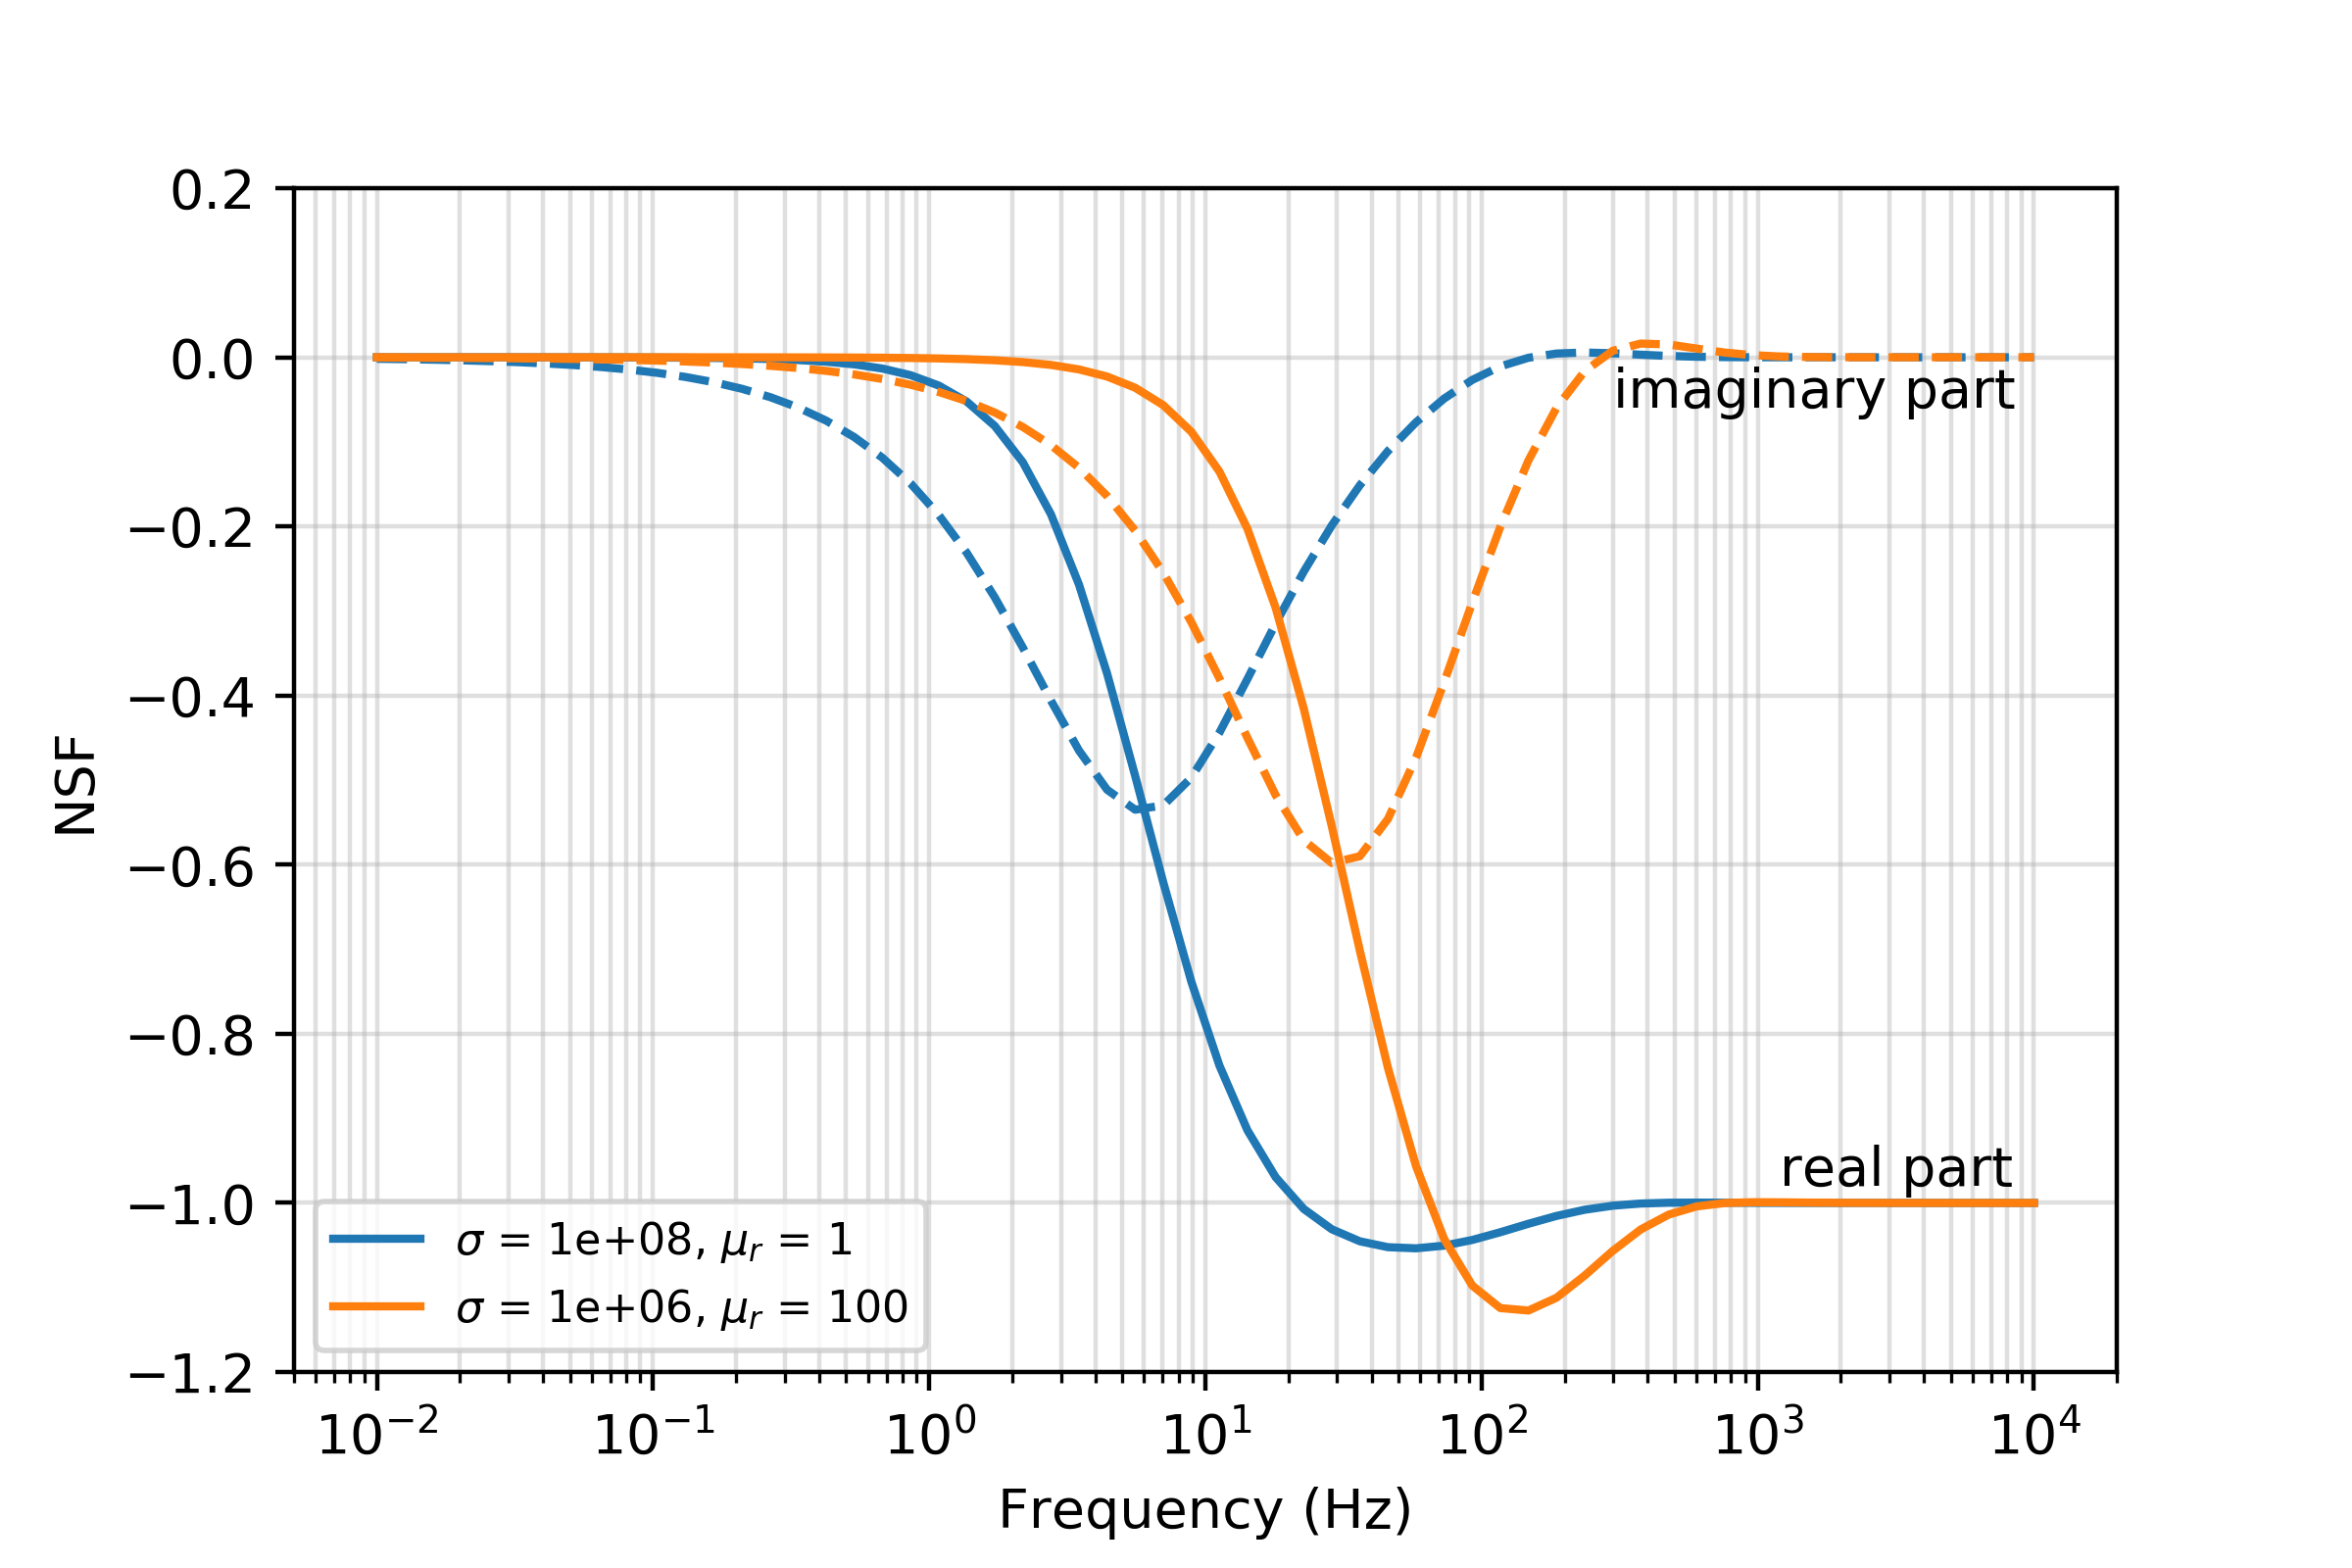
\includegraphics[width=0.6\columnwidth]{figures/casing_software/fdemNSF.png}
    \end{center}
\caption{
    Normalized secondary field, NSF, as a function of frequency for two wells.
    The NSF is the ratio of the secondary vertical magnetic field with the primary magnetic field at the receiver location ($z=$-500 m);
    the primary is defined as the whole-space primary.
}
\label{fig:fdemNSF}
\end{figure}



\begin{figure}
    \begin{center}
    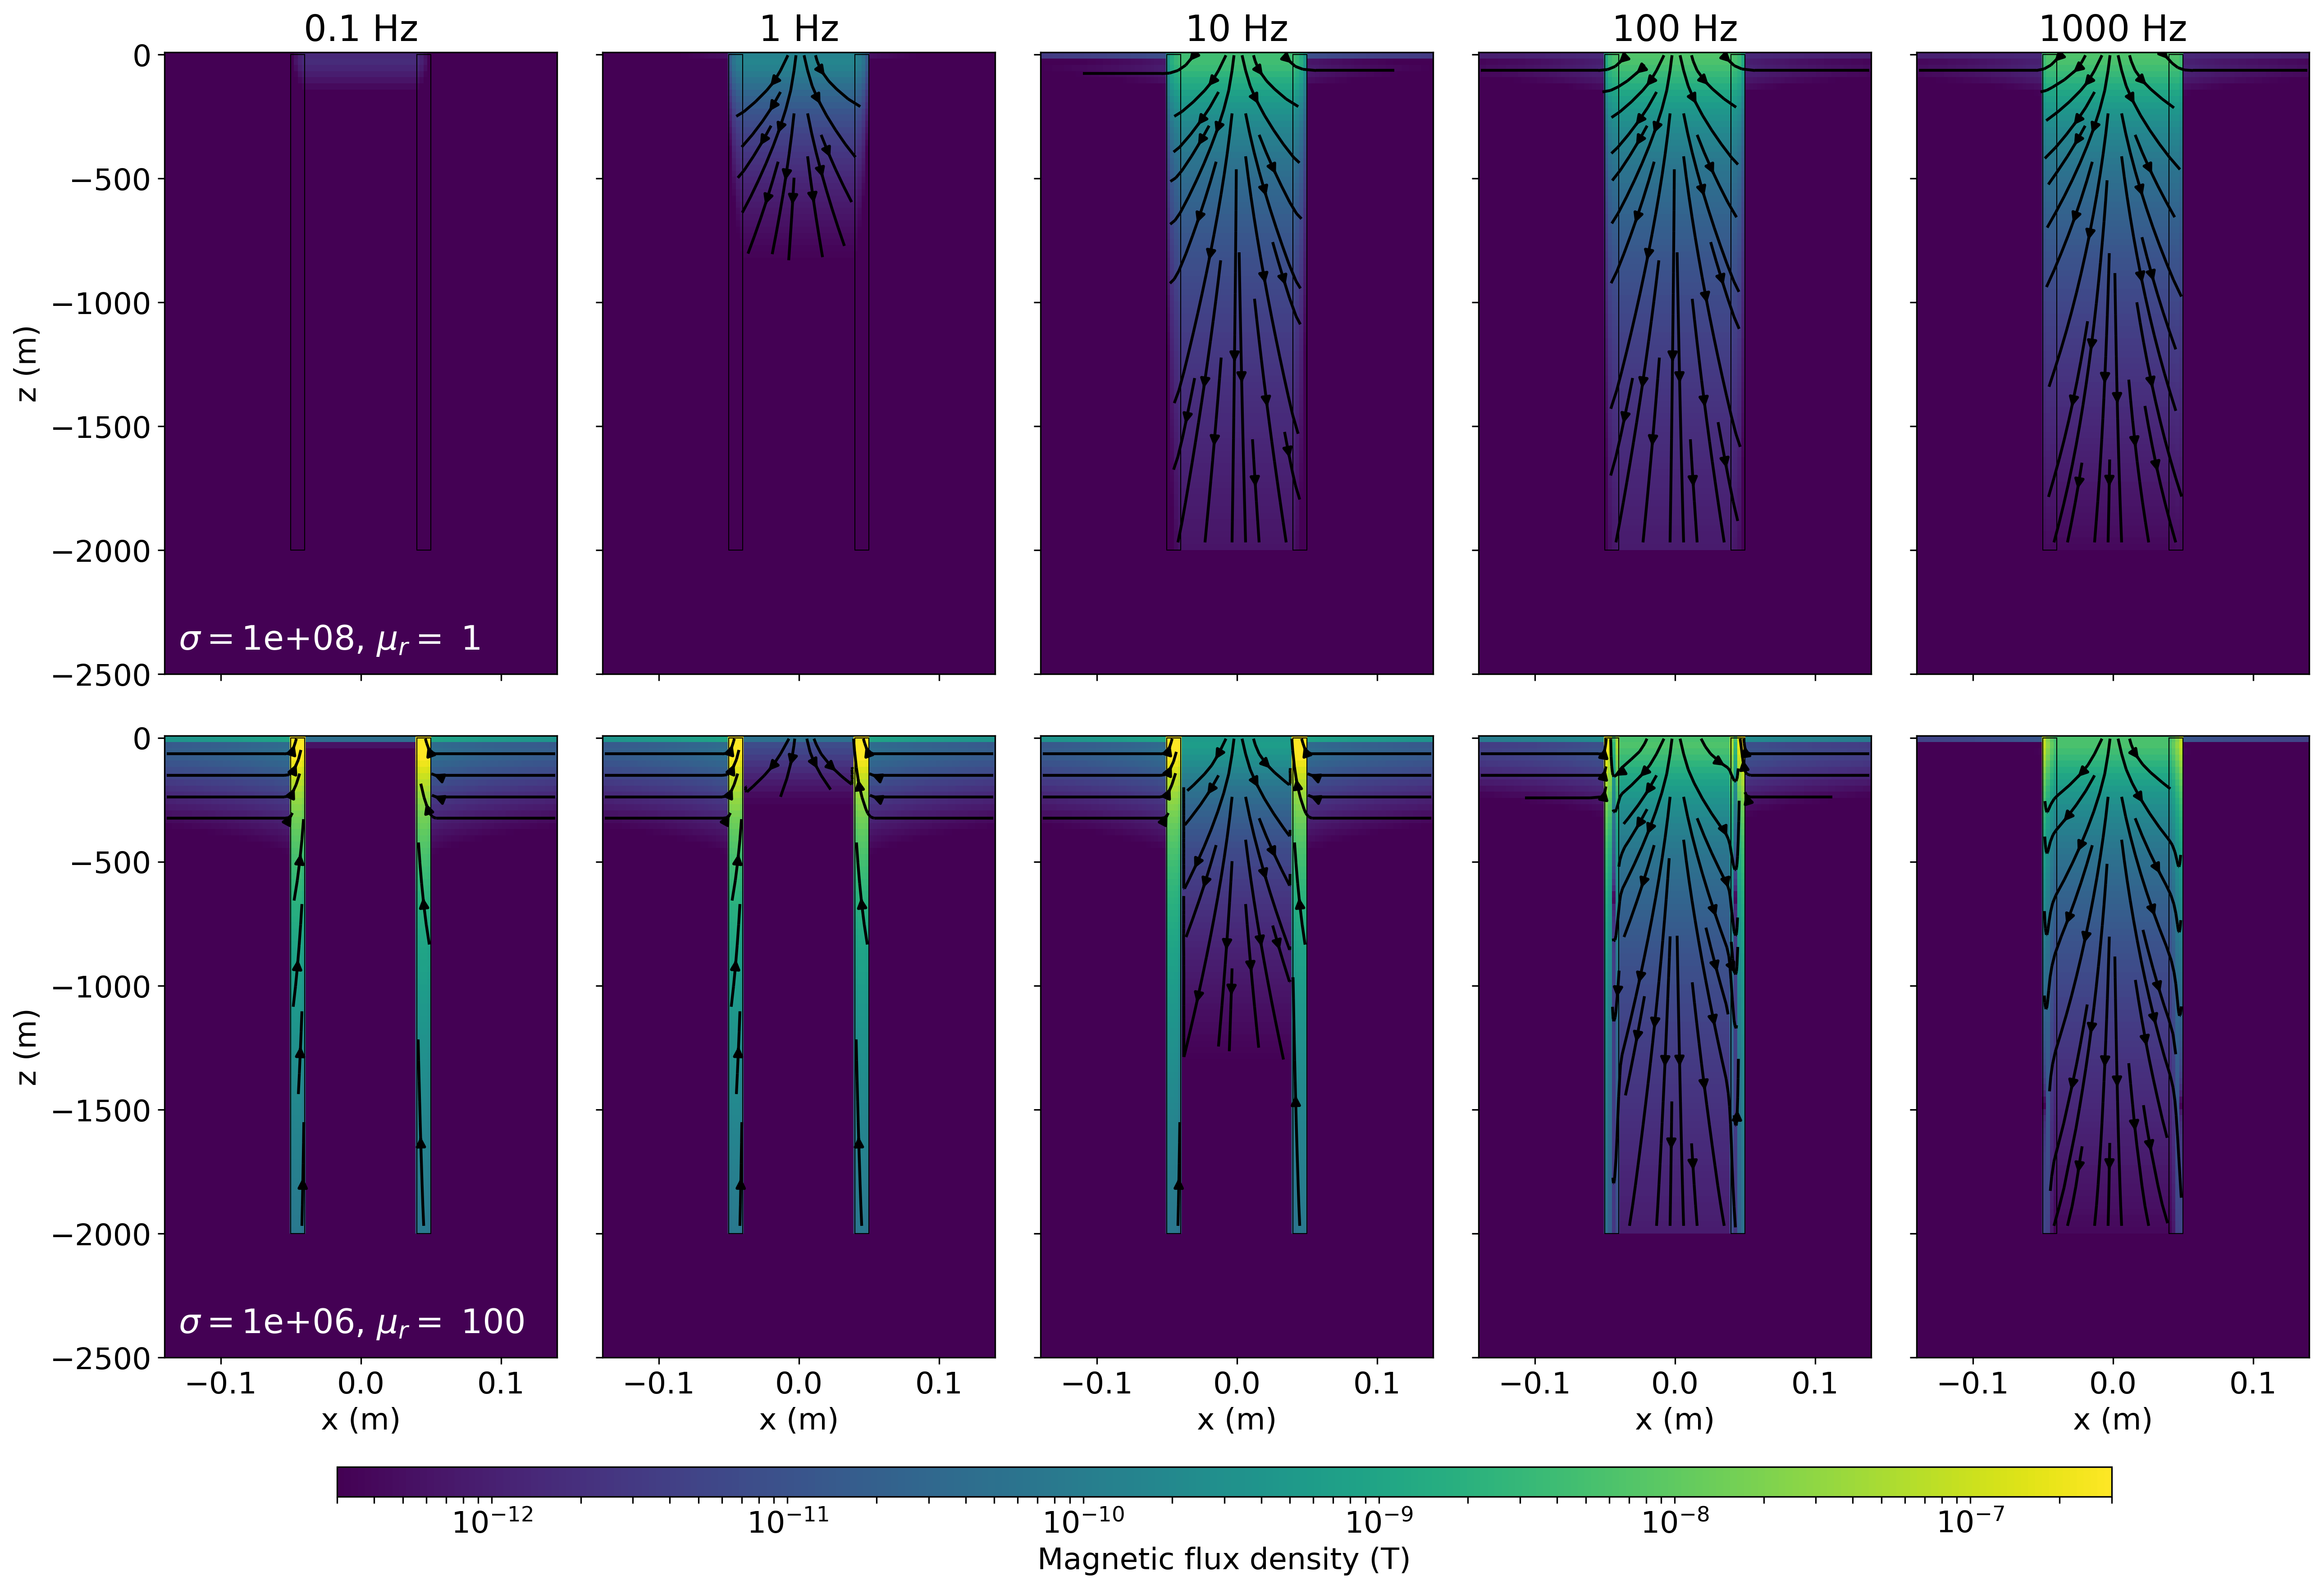
\includegraphics[width=\columnwidth]{figures/bfdem.png}
    \end{center}
\caption{
    Secondary magnetic flux density (with respect to a whole-space primary) at five different frequencies for a conductive pipe (top row)
    and for a conductive, permeable pipe (bottom row).
}
\label{fig:bfdem}
\end{figure}



Conducting a similar experiment in the time domain, we can compare the responses as a function of time. For this experiment, a step-off waveform is employed and data are measured after shut-off, the NSF is plotted in Figure \ref{fig:tdemNSF}. Note here that the secondary field is in the same direction as the primary, so after the source has been shut off, the secondary field is oriented upwards, as shown in Figure \ref{fig:btdem}. Shortly after shut-off, the rate of increase in the secondary field is the same for both the conductive and the conductive, permeable wells. A maximum normalized field strength of approximately 1 is reached for both cases. The responses begin to differ at $10^{-3}$ s where the conductive well maintains a NFS $\sim 1$ for approximately 1 ms longer than the permeable well before the fields decay away.


\begin{figure}[htb]
    \begin{center}
    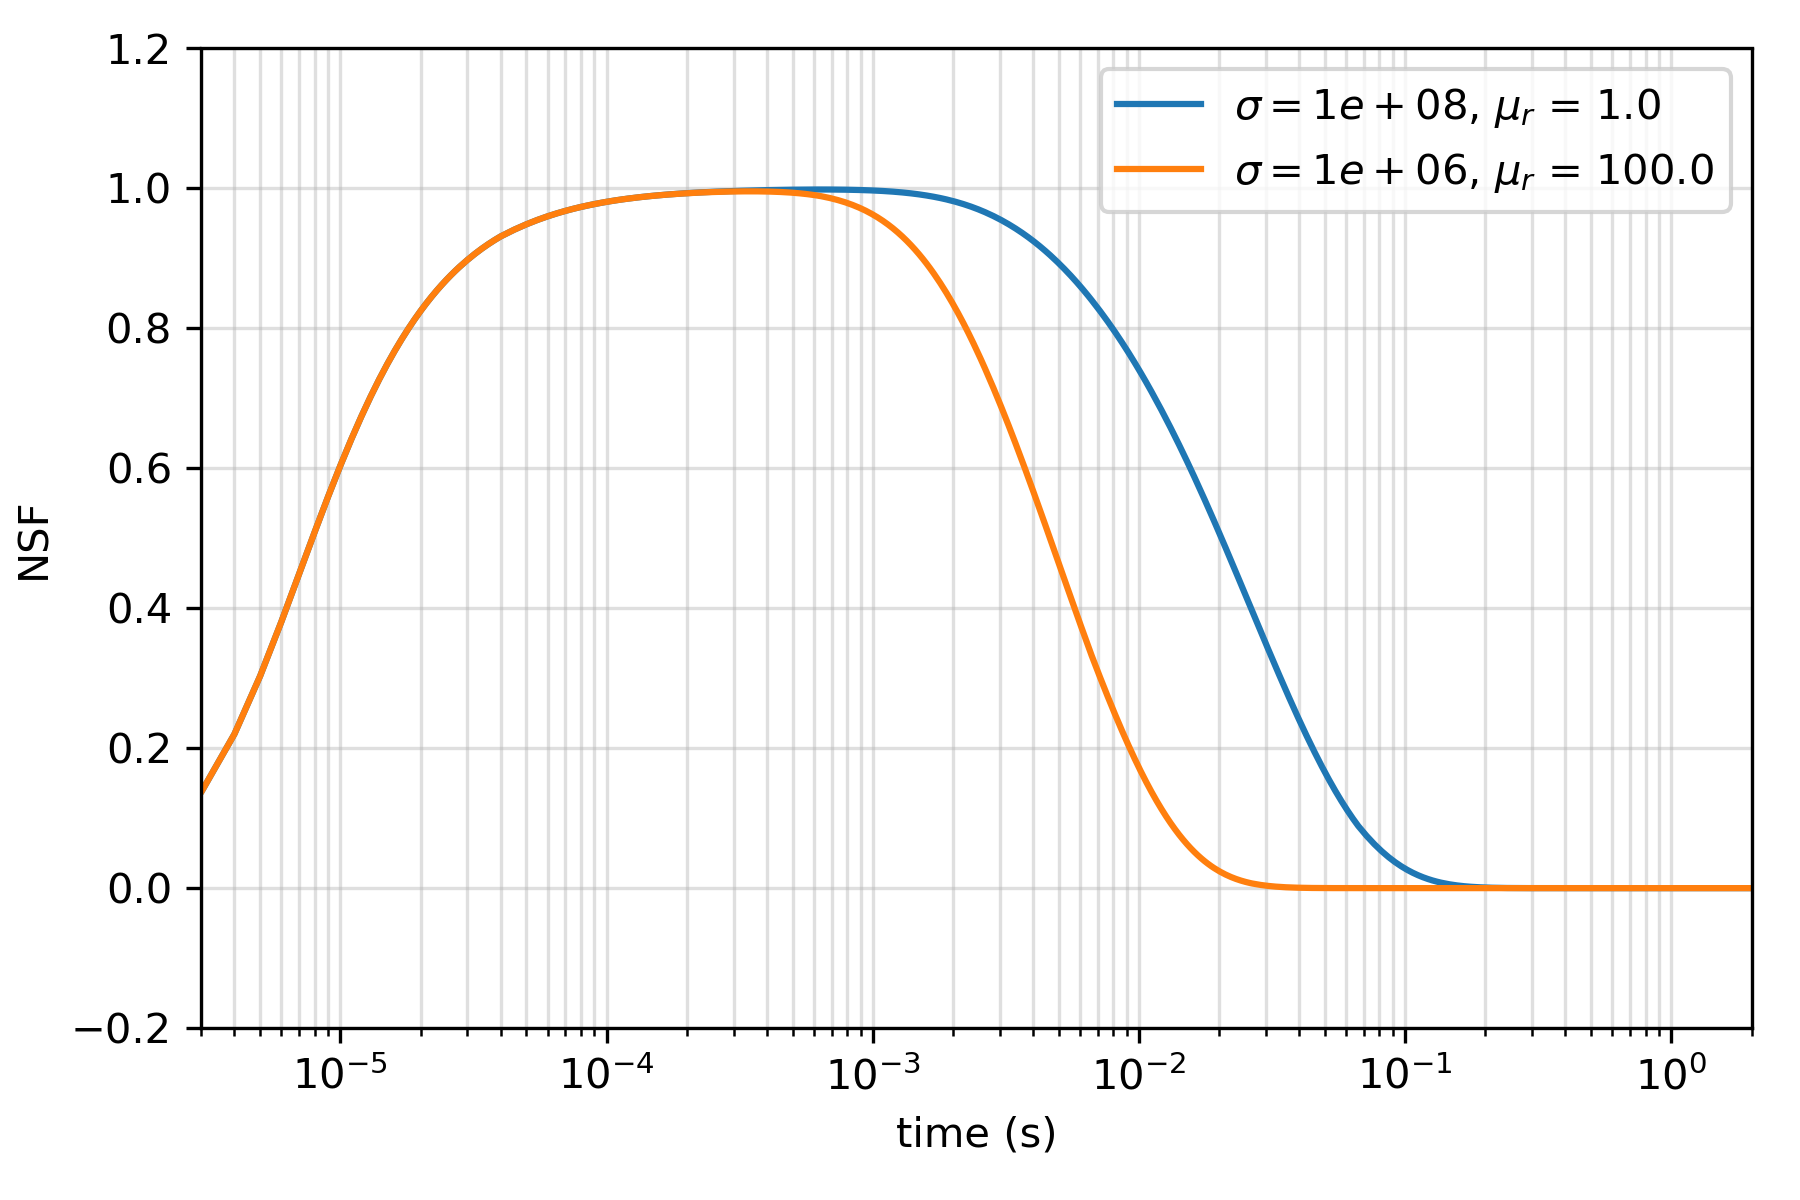
\includegraphics[width=0.6\columnwidth]{figures/tdemNSF.png}
    \end{center}
\caption{
    Normalized secondary field (NSF) through time.
    In the time-domain, we compute the NSF by taking the difference between the total magnetic flux at the reciever and the whole-space response
    and then taking the ratio with the whole-space magnetic flux prior to shutting off the transmitter.
}
\label{fig:tdemNSF}
\end{figure}



\begin{figure}
    \begin{center}
    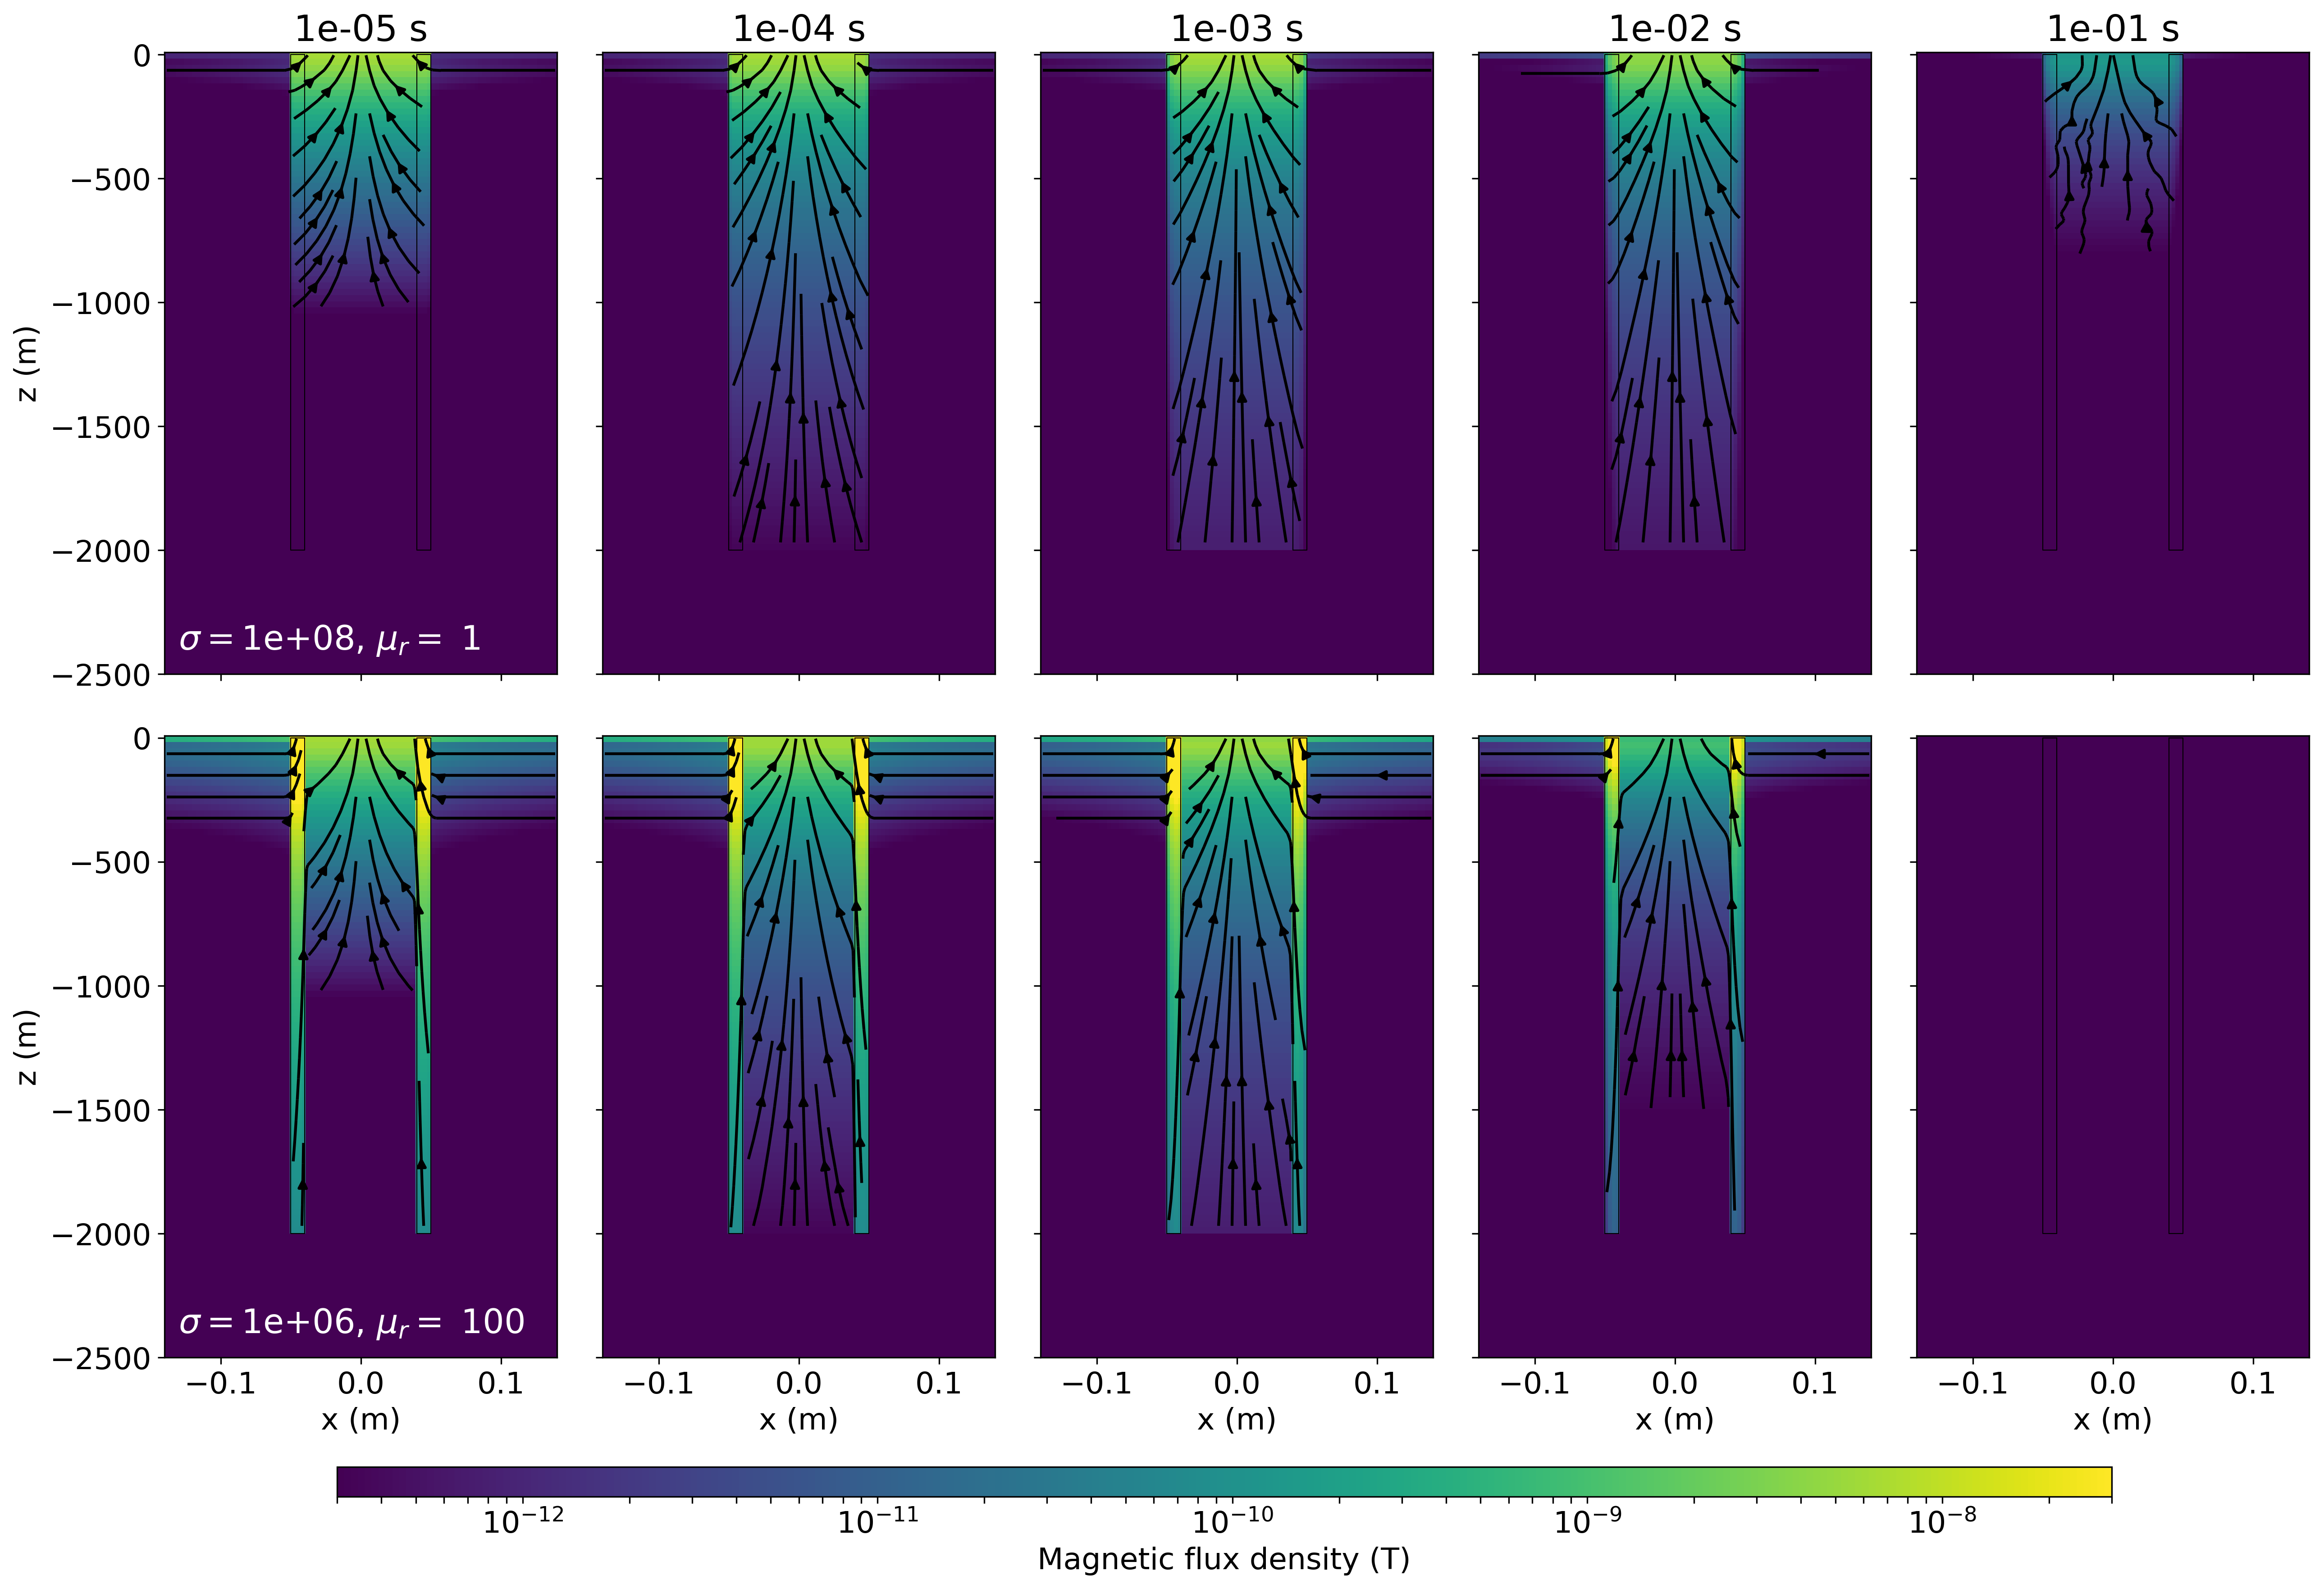
\includegraphics[width=\columnwidth]{figures/casing_software/btdem.png}
    \end{center}
\caption{
    Secondary magnetic flux density for a conductive well (top row) and a conductive, permeable well (bottom row) through time.
    The source waveform is a step-off waveform.
}
\label{fig:btdem}
\end{figure}



\subsubsection{Discussion}

It is important to note that although the product of the conductivity and permeability is identical for these wells, the geometry of the well and inducing fields results in different couplings for each of the parameters. For a vertical magnetic dipole source, the electric fields are purely rotational while the magnetic fields are primarily vertical. An approximation we can use to understand the implications of these geometric differences is to assume the inducing fields are uniform (e.g. the radius of the source loop is infinite) and to examine the conductance and permeance of the pipe. For rotational electric fields, the conductance is
\begin{equation}
    \mathcal{S} = \sigma \frac{t L}{2 \pi r}
    \label{eq:conductance}
\end{equation}

where $t$ is the thickness of the casing, $r$ is the radius of the casing and $L$ is the length-scale of the pipe segment contributing to the signal. For vertical magnetic fields, the permeance is
\begin{equation}
    \mathcal{P} = \mu \frac{ t 2 \pi r}{L}
    \label{eq:permeance}
\end{equation}

As the length-scale, $L$, is larger than the circumference of the pipe ($2\pi r$) the geometric contribution to the conductance is larger than that to the permeance.

An important take-away from this example is that the contributions of conductivity and permeability to the observed EM signals are not simply governed by their product. The geometry of the source fields plays an important role in how each contributes. Thus to accurately model conductive, permeable pipes, over a range of frequencies or times, a numerical code must allow both variable conductivity and variable permeability to be considered.

\section{Summary and Outlook}

I have developed software for solving Maxwell's equations on 2D and 3D cylindrical meshes. The medium can have variable electrical conductivity and magnetic permeability. The 2D solution is especially computationally efficient and has a large number of practical applications. When cylindrical symmetry is not valid, the 3D solution can be implemented; a judicious design of the mesh can often generate a problem with fewer cells than would be required with a tensor or OcTree mesh, thus reducing the computational cost of a simulation. I demonstrated the versatility of the codes by modelling the electromagnetic fields that result when a highly conductive and permeable casing is embedded in the earth.

I presented a number of different experiments involving DC, frequency-domain, and time-domain sources. The first two examples considered a simple DC resistivity experiment. In the first, I demonstrated that the numerically obtained currents, electric fields, and charges emulated those predicted by the asymptotic analysis in \cite{Kaufman1990} for long wells. The second example looked at the transition in behavior of currents and charges between short and long wells. Even in this relatively simple example, the physics was more complex than I originally anticipated; I had not intuitively expected to see the large increase in charge density that was observed near the ends of the well.

In the subsequent examples, I considered electromagnetic experiments and incorporated magnetic permeability in the simulations. I showed that for a conductive and permeable casing, excited by a circular current source, there is a complicated magnetic field that occurs in the top few centimeters of the pipe. Furthermore, the role of conductivity and permeability in the observed responses is more complex than their product; the source geometry and coupling with the casing are important to consider.

As new strategies and software are developed to handle more complex well-geometries, such as deviated or horizontal wells, it is important that we establish an understanding of the physics. Of critical importance is the ability to plot the charges, fields, and fluxes in the simulations. This is valuable for understanding the responses obtained from the experiment and it is a solid foundation for designing a field survey. I anticipate that the software provided with this thesis can be a resource for building understanding and additionally, serve as a tool for testing 3D simulations with boreholes present.

The software implementation is included as a part of the SimPEG ecosystem. SimPEG also includes finite volume simulations on 3D tensor and OcTree meshes as well as machinery for solving inverse problems. This means that the cylindrical codes can be readily connected to an inversion and additionally, simulations and inversions of more complex 3D geologic settings can be achieved by coupling the cylindrical simulation with a 3D tensor or OcTree mesh using a primary-secondary approach (e.g. example 3 in Appendix \ref{app:simpegem}). Beyond modelling steel cased wells, the 3D cylindrical mesh could prove to be useful in conducting 3D airborne EM inversions where a domain-decomposition approach, similar to that described in \cite{Yang2014}, is adopted.

